% !TEX TS-program = xelatex
% Command for running this example (needs latexmkrc file):
%    latexmk -bibtex -pdf main.tex

%	نمونه پایان‌نامه آماده شده با استفاده از کلاس tehran-thesis، نگارش 1
%	سینا ممکن، دانشگاه تهران 
%	https://github.com/sinamomken/tehran-thesis
%	گروه پارسی‌لاتک
%	http://www.parsilatex.com
%	این نسخه، بر اساس نسخه‌ 0.1 از کلاس IUST-Thesis آقای محمود امین‌طوسی آماده شده است.
%        http://profsite.sttu.ac.ir/mamintoosi

%----------------------------------------------------------------------------------------------
% اگر قصد نوشتن پروژه کارشناسی را دارید، در خط زیر به جای msc، کلمه bsc و اگر قصد نوشتن رساله دکترا را دارید، کلمه phd را قرار دهید. کلیه تنظیمات لازم، به طور خودکار، اعمال می‌شود.

% اگر مایلید پایان‌نامه شما دورو باشد به جای oneside در خط زیر از twoside استفاده کنید.

% برای حاشیه‌نویسی و کم کردن صفحات ابتدایی، گزینه draft را وارد و برای نسخه نهایی آن را حذف کنید.

% برای استفاده از قلم‌های سری IR Series گزینه irfonts را وارد و برای استفاده از قلم‌های X Series 2 آن را حذف کنید.

\ExplSyntaxOn
\cs_set_eq:NN
\etex_iffontchar:D
\tex_iffontchar:D
\cs_undefine:N \c_one
\int_const:Nn \c_one { 1 }
\ExplSyntaxOff

\documentclass[
twoside
% ,openany
,msc
,irfonts
% ,draft
]{./tex/tehran-thesis}

% فایل commands.tex را مطالعه کنید؛ چون دستورات مربوط به فراخوانی بسته‌ها، فونت و دستورات خاص در این فایل قرار دارد.
\input{./tex/commands}

% مشخصات پایان‌نامه را در فایلهای faTitle و enTitle وارد نمایید.
% !TeX root=../main.tex
% در این فایل، عنوان پایان‌نامه، مشخصات خود، متن تقدیمی‌، ستایش، سپاس‌گزاری و چکیده پایان‌نامه را به فارسی، وارد کنید.
% توجه داشته باشید که جدول حاوی مشخصات پروژه/پایان‌نامه/رساله و همچنین، مشخصات داخل آن، به طور خودکار، درج می‌شود.
%%%%%%%%%%%%%%%%%%%%%%%%%%%%%%%%%%%%
% دانشگاه خود را وارد کنید
\university{دانشگاه تهران}
% پردیس دانشگاهی خود را اگر نیاز است وارد کنید (مثال: فنی، علوم پایه، علوم انسانی و ...)
\college{پردیس دانشکده‌های فنی}
% دانشکده، آموزشکده و یا پژوهشکده  خود را وارد کنید
\faculty{دانشکده مهندسی برق و کامپیوتر}
% گروه آموزشی خود را وارد کنید (در صورت نیاز)
\department{گروه نرم‌افزار}
% رشته تحصیلی خود را وارد کنید
\subject{مهندسی کامپیوتر}
% گرایش خود را وارد کنید
\field{نرم‌افزار}
% عنوان پایان‌نامه را وارد کنید
\title{کاپو، پلتفرم ساخت و انتقال توکن‌های داده‌ای}
% نام استاد(ان) راهنما را وارد کنید
\firstsupervisor{دکتر احسان خامس‌پناه}
\firstsupervisorrank{استاد}
% \secondsupervisor{دکتر راهنمای دوم}
% \secondsupervisorrank{استادیار}
% نام استاد(دان) مشاور را وارد کنید. چنانچه استاد مشاور ندارید، دستورات پایین را غیرفعال کنید.
% \firstadvisor{دکتر مشاور اول}
\firstadvisorrank{استادیار}
%\secondadvisor{دکتر مشاور دوم}
% نام داوران داخلی و خارجی خود را وارد نمایید.
\internaljudge{دکتر محمد صیادحقیقی}
\internaljudgerank{استاد}
% \externaljudge{دکتر داور خارجی}
% \externaljudgerank{دانشیار}
% \externaljudgeuniversity{دانشگاه داور خارجی}
% نام نماینده کمیته تحصیلات تکمیلی در دانشکده \ گروه
\graduatedeputy{دکتر نماینده}
\graduatedeputyrank{دانشیار}
% نام دانشجو را وارد کنید
\name{امین}
% نام خانوادگی دانشجو را وارد کنید
\surname{بشیری}
% شماره دانشجویی دانشجو را وارد کنید
\studentID{810196425}
% تاریخ پایان‌نامه را وارد کنید
\thesisdate{خرداد ۱۴۰۱}
% به صورت پیش‌فرض برای پایان‌نامه‌های کارشناسی تا دکترا به ترتیب از عبارات «پروژه»، «پایان‌نامه» و «رساله» استفاده می‌شود؛ اگر  نمی‌پسندید هر عنوانی را که مایلید در دستور زیر قرار داده و آنرا از حالت توضیح خارج کنید.
%\projectLabel{پایان‌نامه}

% به صورت پیش‌فرض برای عناوین مقاطع تحصیلی کارشناسی تا دکترا به ترتیب از عبارت «کارشناسی»، «کارشناسی ارشد» و «دکتری» استفاده می‌شود؛ اگر نمی‌پسندید هر عنوانی را که مایلید در دستور زیر قرار داده و آنرا از حالت توضیح خارج کنید.
%\degree{}
%%%%%%%%%%%%%%%%%%%%%%%%%%%%%%%%%%%%%%%%%%%%%%%%%%%%
%% پایان‌نامه خود را تقدیم کنید! %%
% \dedication
% {
% {\Large تقدیم به:}\\
% \begin{flushleft}{
% 	\huge
% 	همسر و فرزندانم\\
% 	\vspace{7mm}
% 	و\\
% 	\vspace{7mm}
% 	پدر و مادرم
% }
% \end{flushleft}
% }
%% متن قدردانی %%
%% ترجیحا با توجه به ذوق و سلیقه خود متن قدردانی را تغییر دهید.
% \acknowledgement{
% سپاس خداوندگار حکیم را که با لطف بی‌کران خود، آدمی را به زیور عقل آراست.

% در آغاز وظیفه‌  خود  می‌دانم از زحمات بی‌دریغ اساتید  راهنمای خود،  جناب آقای دکتر ... و ...، صمیمانه تشکر و  قدردانی کنم که در طول انجام این پایان‌نامه با نهایت صبوری همواره راهنما و مشوق من بودند و قطعاً بدون راهنمایی‌های ارزنده‌ ایشان، این مجموعه به انجام نمی‌رسید.

% از جناب آقای دکتر ... که  زحمت مشاوره‌، بازبینی و تصحیح این پایان‌نامه را تقبل فرمودند کمال امتنان را دارم.

% %از همکاری و مساعدت‌های دکتر ... مسئول تحصیلات تکمیلی و سایر کارکنان دانشکده بویژه سرکار خانم ... کمال تشکر را دارم.

% با سپاس بی‌دریغ خدمت دوستان گران‌مایه‌ام، خانم‌ها ... و آقایان ... در آزمایشگاه ...، که با همفکری مرا صمیمانه و مشفقانه یاری داده‌اند.

% و در پایان، بوسه می‌زنم بر دستان خداوندگاران مهر و مهربانی، پدر و مادر عزیزم و بعد از خدا، ستایش می‌کنم وجود مقدس‌شان را و تشکر می‌کنم از خانواده عزیزم به پاس عاطفه سرشار و گرمای امیدبخش وجودشان، که بهترین پشتیبان من بودند.
% }
%%%%%%%%%%%%%%%%%%%%%%%%%%%%%%%%%%%%
%چکیده پایان‌نامه را وارد کنید
\fa-abstract{

هدف از انجام این پروژه ساخت پلتفرمی متن‌باز
\LTRfootnote{\url{https://github.com/bshramin/cappu}}
به نام کاپو است که هر شخص یا شرکتی بتواند با عضویت در آن،
به آسان‌ترین روش ممکن توکن‌های تعویض‌ناپذیر‌ بسازد و به دیگران انتقال دهد.
این پلتفرم کاربردهای فراوانی دارد.
دارایی‌هایی مانند بلیت سینما، ژتون‌های غذا، وقت گرفتن از دکتر، قراردادها و ... همه
می‌توانند به آسانی در این پلتفرم به توکن تعویض‌ناپذیر تبدیل شوند،
به دیگران انتقال یابند و در بازار خرید و فروش شوند.

گرچه می‌توان کاربردهای فراوانی را برای این پلتفرم در نظر داشت
اما همچنان یکی از اهداف انجام این پروژه آشنایی با نحوه ساخت، آزمون و بارگذاری یک قرارداد هوشمند،
ساخت واسط‌کاربری و اتصال آن به قرارداد هوشمند،
و همچنین شناخت استاندارد‌های معروف قرارداد‌های توکن‌های تعویض‌ناپذیر مانند
\lr{ERC721}
و
\lr{ERC1155}
است.

\gls{Decentralized Web}
یا
\lr{Web3}
 به عنوان مهم‌ترین تغییر بعد از به وجود آمدن
\gls{Word Wide Web}
 در نظر گرفته می‌شود. با به وجود آمدن
\glspl{CryptoCurrency}
و
\glspl{Consensus Algorithms}
کارآمد، و فراهم شدن زمینه اجرای برنامه‌ها و انجام تراکنش‌های مالی به صورت غیر متمرکز،
عصر اینترنت غیرمتمرکز فرا رسیده است.

در این میان یکی از اصلی‌ترین مزایای 
\glspl{Dapp}
مالکیت واقعی دارایی است.
به این معنی که یک شخص یا یک نهاد نمی‌تواند دارایی‌های کس دیگری را مسدود یا مصادره کند.
همچنین مالیکت‌های معنوی نیز به صورت واضح و شفاف می‌توانند مشخص شوند.
برای مثال یک هنرمند به وضوح صاحب اثرش است و هرچند که دیگر افراد می‌توانند اثر او را کپی کنند
اما همیشه مشخص است که صاحب اصلی اثر کیست.

به این ترتیب 
\glspl{Non-fungible token}
با قابلیت‌های بسیار زیادی که فراهم می‌کنند مورد استقبال فراوان مردم واقع شدند.
قابلیت‌هایی مانند ساخت، نگهداری، فروش و انتقال فوق‌العاده راحت و سریع نیز
در این سرعت فراگیری تاثیر بسزایی داشته‌اند.
برای این بازار تازه و بزرگ، تکنولوژی‌ها، استاندارد‌ها و پلتفرم‌های زیادی ساخته شده‌اند
و همچنان نیز در حال توسعه هستند.
}
% کلمات کلیدی پایان‌نامه را وارد کنید
\keywords{
کاپو،
توکن،
داده،
سالیدیتی،
قرارداد هوشمند،
توکن غیرقابل تعویض،
ترافل
}
% انتهای وارد کردن فیلد‌ها
%%%%%%%%%%%%%%%%%%%%%%%%%%%%%%%%%%%%%%%%%%%%%%%%%%%%%%

% مشخصات انگلیسی پایان‌نامه
% !TeX root=../main.tex
% در این فایل، عنوان پایان‌نامه، مشخصات خود و چکیده پایان‌نامه را به انگلیسی، وارد کنید.

%%%%%%%%%%%%%%%%%%%%%%%%%%%%%%%%%%%%
\latinuniversity{University of Tehran}
\latincollege{College of Engineering}
\latinfaculty{Faculty of Electrical and Computer Engineering}
\latindepartment{Software Department}
\latinsubject{Computer Engineering}
\latinfield{Software Engineering}
\latintitle{Cappu, a platform to mint and transfer data NFTs.}
\firstlatinsupervisor{Dr. Ehsan Khamespanah}
% \secondlatinsupervisor{Second Supervisor}
% \firstlatinadvisor{First Advisor}
%\secondlatinadvisor{Second Advisor}
\latinname{Amin}
\latinsurname{Bashiri}
\latinthesisdate{June 2022}
\latinkeywords{Cappu, NFT, smart-contract, solidity, ERC721}
\en-abstract{ % TODO:
This thesis studies on writing projects, theses and dissertations using tehran-thesis class. It ...
}


% تنظیمات و تعاریف واژه‌نامه و اختصارات
\input{./tex/glossaries-settings}
\newword{Word Wide Web}{Word Wide Web}{اینترنت}{}

\newword{Fiat Money}{Fiat Money}{پول فیزیکی}{}

\newword{Decentralized Web}{Decentralized Web}{اینترنت غیرمتمرکز}{}

\newword{CryptoCurrency}{CryptoCurrencies}{رمزارز}{رمزارزها}

\newword{Private key}{Private key}{کلید خصوصی}{کلید خصوصی}

\newword{Mint}{Mint}{ساخت}{}

\newword{Settings}{Settings}{تنظیمات}{تنظیمات}

\newword{Network}{Networks}{شبکه}{شبکه‌ها}

\newword{State}{State}{حالت}{}

\newword{Developer}{Developers}{توسعه‌دهنده}{توسعه‌دهندگان}

\newword{Decompiler}{}{دیکامپایلر}{}

\newword{bytecode}{bytecodes}{بایت‌کد}{بایت‌کدها}

\newword{Confidentiality}{Confidentiality}{محرمانگی}{}

\newword{Consensus Algorithms}{Consensus Algorithms}{الگوریتم اجماع}{الگوریتم‌های اجماع}

\newword{Non-fungible}{Non-fungibles}{تعویض ناپذیر}{تعویض ناپذیرها}

\newword{Non-fungible token}{Non-fungible tokens}{توکن تعویض ناپذیر}{توکن‌های تعویض ناپذیر}

\newword{Dapp}{Dapps}{برنامه غیرمتمرکز}{برنامه‌های غیرمتمرکز}

\newword{Smart Contract}{Smart Contracts}{قرارداد هوشمند}{قراردادهای هوشمند}

\newword{Testnet}{Testnets}{شبکه تستی}{شبکه‌های تستی}

\newword{Mainnet}{Mainnets}{شبکه اصلی}{شبکه‌های اصلی}

\newword{Github Pages}{Github Pages}{صفحات گیت‌هاب}{}

\newword{Wallet}{Wallets}{کیف پول دیجیتال}{کیف پول‌های دیجیتال}

\newword{Open Source}{Open Source}{متن‌باز}{}

\newword{OpenZeppelin}{OpenZeppelin}{اپن‌زپلین}{}

\newword{Login}{Login}{ورود}{ورود}

\newword{Logout}{Logout}{خروج}{خروج}

\newword{Block Explorer}{Block Explorers}{جستجوگر شبکه}{جستجوگرهای شبکه}

\newword{Automatic}{Automatic}{خودکار}{}

\newword{Dockerize}{Dockerize}{داکرایز}{}

\newword{Truffle}{Truffle}{ترافل}{}

\newword{Docker Image}{Docker Images}{ایمیج داکر}{ایمیج‌های داکر}

\newword{Platform}{Platforms}{پلتفرم}{پلتفرم‌ها}

\newword{Develop}{Develop}{توسعه}{}

\newword{Gloss}{Glossary}{واژه‌نامه}{واژه‌نامه‌ها}

\newword{Acronym}{Acronym}{اختصار}{اختصارات}

\newword{Ropsten}{Ropsten}{راپستن}{راپستن}

\newword{Description}{Description}{توصیف}{توصیف‌ها}

\newword{Draft}{Draft}{پیش‌نویس}{پیش‌نویس‌ها}

\newword{Absorption}{Absorption}{جذب}{جذب‌ها}

\newword{RandomVariable}{Random Variable}{متغیر تصادفی}{متغیرهای تصادفی}

\newword{Action}{Action}{کنش}{کنش‌ها}

\newword{Mnemonics}{Mnemonics}{نمونیکز}{نمونیکز}

\newword{Optimization}{Optimization}{بهینه‌سازی}{}

\newword{Drizzle}{Drizzle}{دریزل}{دریزل}

\newword{Framework}{Frameworks}{چارچوب}{چارچوب‌ها}

\newword{Community}{Community}{جامعه توسعه‌دهندگان}{جامعه توسعه‌دهندگان}

\input{./tex/acronyms}

\begin{document}

\pagenumbering{adadi} % یک، دو، ...
% ابتدای درج صفحات مختلف
\coverPage
% بررسی حالت پیش‌نویس
\ifoptiondraft{}{% 
    \besmPage
    \titlePage
    \davaranPage
%%%%%%%%%%%%%%%%%%%%%%%%%%%
    \esalatPage
    % \mojavezPage
% چنانچه مایل به چاپ صفحات «تقدیم»، «نیایش» و «سپاس‌گزاری» در خروجی نیستید، خط‌های زیر را با گذاشتن ٪  در ابتدای آنها غیرفعال کنید.
    % \taghdimPage
    % \ghadrdaniPage
} % end ifoptiondraft
\abstractPage
% شروع درج فهرست‌ها
\newpage\cleardoublepage
\pagenumbering{harfi} % آ، ب، ...
\tableofcontents \clearpage
% بررسی حالت پیش‌نویس برای بقیه فهرست‌ها
\ifoptiondraft{
    \listoftodos
}{%
    % \listoffigures \clearpage
    % \listoftables  \clearpage
    % \addcontentsline{toc}{chapter}{\listalgorithmname}
    % \listofalgorithms \clearpage
    % \addcontentsline{toc}{chapter}{\lstlistlistingname}
    \lstlistoflistings \clearpage
    % \printacronyms
} % end ifoptiondraft

\pagestyle{fancy}
\pagenumbering{arabic} % 1, 2, ...

% !TeX root=../main.tex

\chapter{مقدمه و بیان مسئله}
% دستور زیر باعث عدم‌نمایش شماره صفحه در اولین صفحهٔ این فصل می‌شود.
%\thispagestyle{empty}

% ------------ Section 1.1 ------------
\section{مقدمه}
در یک دهه اخیر محبوبیت رمزارز‌ها در میان مردم به شدت افزایش داشته است. رمزارزها توکن هایی تعویض پذیر هستند به این معنی که تفاوتی میان دو توکن یک
\gls{CryptoCurrency}
وجود ندارد، مانند
\gls{Fiat Money}
که ارزش یک هزار تومانی با یک هزار تومانی دیگر تفاوتی ندارد.

اما در دنیای واقعی تنها مالکیت پول نیست که اهمیت دارد، بلکه یک فرد می‌تواند خودرو، خانه، بلیت هواپیما و دیگر دارایی‌هایی داشته باشد که یکتا هستند و با هیچ دارایی دیگری دقیقا یکسان نیستند. مثلا یک بلیت هواپیما برای تاریخ و ساعتی خاص برای شماره پروازی خاص از یک مبدا مشخص به یک مقصد مشخص است و شماره صندلی یکتایی نیز دارد. پس هیچ دو بلیت هواپیمایی دقیقا یکسان نیستند، بر خلاف دو بیتکوین که کاملا یکسان هستند، ارزش برابری دارند، و تعویض پذیر هستند.

کاربردهای توکن‌های تعویض ناپذیر بیشمار است و در حال حاضر فقط قسمت اندکی از کاربردهایی که می‌توانند داشته باشند را پاسخ گفته‌اند. در این پروژه یک
\gls{Platform}
می‌سازیم که ساخت و انتقال توکن‌های تعویض ناپذیر را برای عموم در دسترس‌تر و آسان‌تر می‌کند. همچنین یکی از اهداف انجام این پروژه آشنایی با تکنولوژی‌ها، استاندارد‌ها و فرایند‌های توسعه این توکن‌هاست.


% ------------ Section 1.2
\section{شرح مسئله و روش انجام آن}
پروژه تعریف شده توسعه یک پلتفرم برای
\gls{Mint}
و انتقال توکن‌های تعویض ناپذیر به آسان‌ترین روش ممکن است، به نحوی که برای هر کسی به راحتی در دسترس باشد. نکته‌ی قابل توجه‌ این است که در مسیر انجام این پروژه با تکنولوژی‌های موجود در این زمینه، فریمورک‌ها، استاندارد‌ها و فرایند تست و دیپلوی آشنا شویم.

برای انجام این مراحل در قدم اول نحوه توسعه اپلیکیشن‌های غیرمتمرکز و برتری‌های نوشتن پروژه به صورت متن‌باز ذکر می‌شود، سپس فریمورک‌ها و ابزار‌هایی که برای ساخت یک اپلیکیشن غیرمتمرکز به توسعه دهنده کمک می‌کنند معرفی می‌شوند و نحوه استفاده از آن‌ها شرح داده می‌شود.

سپس فرایند توسعه آغاز می‌شود، استاندارد‌های موجود برای نوشتن یک قرارداد برای توکن‌های تعویض ناپذیر شرح داده می‌شود و کاپو تا جای ممکن مطابق آن‌ها توسعه می‌یابد. برای قرارداد هوشمند نوشته شده تست می‌نویسیم و آن را روی
\gls{Testnet}
انتشار می‌دهیم.
در گام بعد برای پلتفرم، فرانت‌اند ساده‌ای نوشته می‌شود که با قرارداد هوشمند و همچنین کیف پول دیجیتال کاربر ارتباط برقرار می‌کند و سپس به کمک
\gls{Github Pages}
دیپلوی می‌شود تا در دسترس عموم کاربرها قرار بگیرد.

برای
\gls{Dockerize}
کردن تست‌های
\gls{Smart Contract}
یک
\gls{Docker Image}
\gls{Truffle}
نوشته می‌شود. در قدم بعد هر دو بخش فرانت و قرارداد هوشمند داکرایز می‌شوند و فرایند اجرای تست‌های قرارداد هوشمند و دیپلوی شدن فرانت به صورت خودکار به کمک پایپلاین‌های گیت‌هاب پیاده‌سازی می‌شود.


% ------------ Section 1.3
\section{اهداف کلی تحقیق}
اهداف این تحقیق را می‌توان به دو دسته تقسیم‌بندی نمود.

\subsection{گسترش کاربرد‌های توکن‌های تعویض ناپذیر}
این توکن‌ها در همین مدت کوتاهی که به وجود آمده‌اند کاربردهای فراوانی را پوشش داده‌اند. اما همچنان قسمت بزرگی از این کاربردها صرفا ثبت مالکیت آثار هنری دیجیتال است. درحالی که توکن‌های داده‌ای می‌توانند وسعت بسیار عظیم‌تری از کاربردها را پوشش دهند. از کاربردهای روزانه مانند بلیت سینما و هواپیما، تا مالکیت هر نوع دارایی واقعی یا مجازی.

با توجه به نحوه کار اکثر قراردادهای توکن‌های تعویض ناپذیر، معمولا فقط مالک قرارداد می‌تواند توکن ایجاد کند، یا در قرارداد برای ایجاد توکن شرط‌هایی مانند حداکثر تعداد ممکن گذاشته می‌شود. این موضوع به این معنی است که اگر شخصی بخواهد خودش توکن‌هایی ایجاد کند و به دیگران انتقال دهد احتمالا مجبور است که قراردادهوشمند خودش را بنویسد و دیپلوی کند. این فرآیند نیاز به دانش فنی، آشنایی کامل با این زمینه و پرداخت هزینه‌های دیپلوی قرارداد روی شبکه بلاکچین دارد.

کاپو به هر آدرسی اجازه می‌دهد که به راحت‌ترین حالت ممکن و به هر تعداد که مورد نیاز است توکن تعویض ناپذیر روی این قرارداد ایجاد کند. به این ترتیب استفاده از کاپو برای عموم مردم آسان‌تر، ارزان‌تر و در دسترس‌تر است.

\subsection{یادگیری}
هدف دیگر انجام این پروژه یادگیری است. با توجه به رشد سریع و تازگی استفاده از تکنولوژی‌های بلاکچین و توکن‌های تعویض ناپذیر، با وجود تلاش برای ایجاد منابع یادگیری مناسب همچنان فضاهای خالی، کمبودها و نیازمندی‌هایی وجود دارد که باید پاسخ گفته شوند. در طی انجام این پروژه با ابزارها، کتابخانه‌ها، فریمورک‌ها و استانداردهای نوشتن قراردادهای هوشمند آشنا می‌شویم، می‌آموزیم که هر یک چطور کار میکنند و چگونه می‌توانند به توسعه دهنده کمک کنند.

% ------------ Section 1.4
\section{ساختار پایان‌نامه}
پس از این مقدمه، در فصل ۲ مفاهیم اولیه توسعه اپلیکیشن بر بستر بلاک‌چین، کاربردها، مفاهیم و استاندارد‌ها توضیح داده می‌شود. در فصل ۳ ابزار‌های توسعه قرارداد‌های هوشمند معرفی می‌شوند، مزایا و معایب هر یک بیان می‌شود و نحوه استفاده از آن‌ها توضیح داده می‌شود. در فصل ۴ روند پیاده‌سازی شرح داده می‌شود. بررسی می‌شود که در هر مرحله از پیاده‌سازی چه کارهایی به چه ترتیبی انجام شده است. در فصل پنجم نیز نتایج توضیح داده می‌شوند و جمع‌بندی صورت میگیرد.
		% فصل اول: مقدمه
% !TeX root=../main.tex
\chapter{مفاهیم اولیه و پیش‌زمینه}
% ------------ Section 2.1
\section{دلایل و برتری‌های متن‌باز بودن قرارداد‌های هوشمند}
دلایل زیادی برای متن‌باز نوشتن قراردادهای هوشمند وجود دارد، در ادامه تعدادی از این دلایل توضیح داده می‌شود.

دلیل اول، بلاک‌چین‌ها
\gls{Confidentiality}
ندارند، همه‌ی نود‌های شبکه برای اجرای کد قرارداد هوشمند باید حداقل به
\glspl{bytecode}
قرارداد هوشمند دسترسی داشته باشند و این بایت‌کد‌ها در کاوشگرهای بلاکچین نیز وجود دارند، همچنین
\gls{Decompiler}هایی
وجود دارند که از بایت‌کد‌های قرارداد هوشمند کد سالیدیتی آن را به دست می‌آورند. پس در نتیجه تلاش برای مخفی کردن کدهای قرارداد هوشمند بیهوده خواهد بود.

دلیل دوم، اصلی‌ترین مزیت اپلیکیشن‌های غیرمتمرکز نسبت به اپلیکیشن‌های متمرکز عدم نیاز به اعتماد است، کاربرها می‌توانند کد‌های قرارداد هوشمند را بخوانند و به کد نوشته شده اعتماد کنند،‌در حالی که اگر کد برنامه برای همه کاربران قابل مشاهده نباشد کاربرها باید به سازندگان آن برنامه اعتماد کنند.

دلیل سوم، بارگذاری کردن قرارداد‌های هوشمند معمولا آسان نیست و سرعت تغییرات پایین‌تر از اپلیکیشن‌های متمرکز هست،‌ پس امکان این که با پیدا شدن هر مشکل بتوان به سرعت آن را درست کرد کمتر وجود دارد و مسئله امنیت بسیار اهمیت دارد. متن‌باز نوشتن قرارداد هوشمند باعث می‌شود چشم‌های بیشتری کدهای قرارداد را بخوانند و مشکلات احتمالی سریعتر مشخص و رفع شوند. تعداد زیادی از این پروژه‌ها از همان روز اول قرارداد هوشمند را به صورت متن‌باز توسعه می‌دهند، بعضی نیز ترجیح میدهند که پروژه به مرحله‌ای از توسعه برسد و سپس آن را متن‌باز میکنند.

ر این حوضه سرعت پیشرفت و توسعه به دلیل متن باز بودن به شدت بالاست به نحوی که در طی اجرای این پروژه مرج ریکوئستی روی کتابخانه OpenZeppelin زده شد که در همان روز مرج شد. این موضوع علاوه بر این که نشان‌دهنده سرعت پیشرفت بسیار بالاست، این موضوع را نیز نشان میدهد که در یک جامعه متن‌باز هر توسعه دهنده می‌تواند به پیشرفت جامعه به هر شکلی که می‌تواند کمک کند، اشکالاتی که مشاهده می‌کند را گزارش دهد یا تصحیح کند.

\begin{figure}[ht]
\centerline{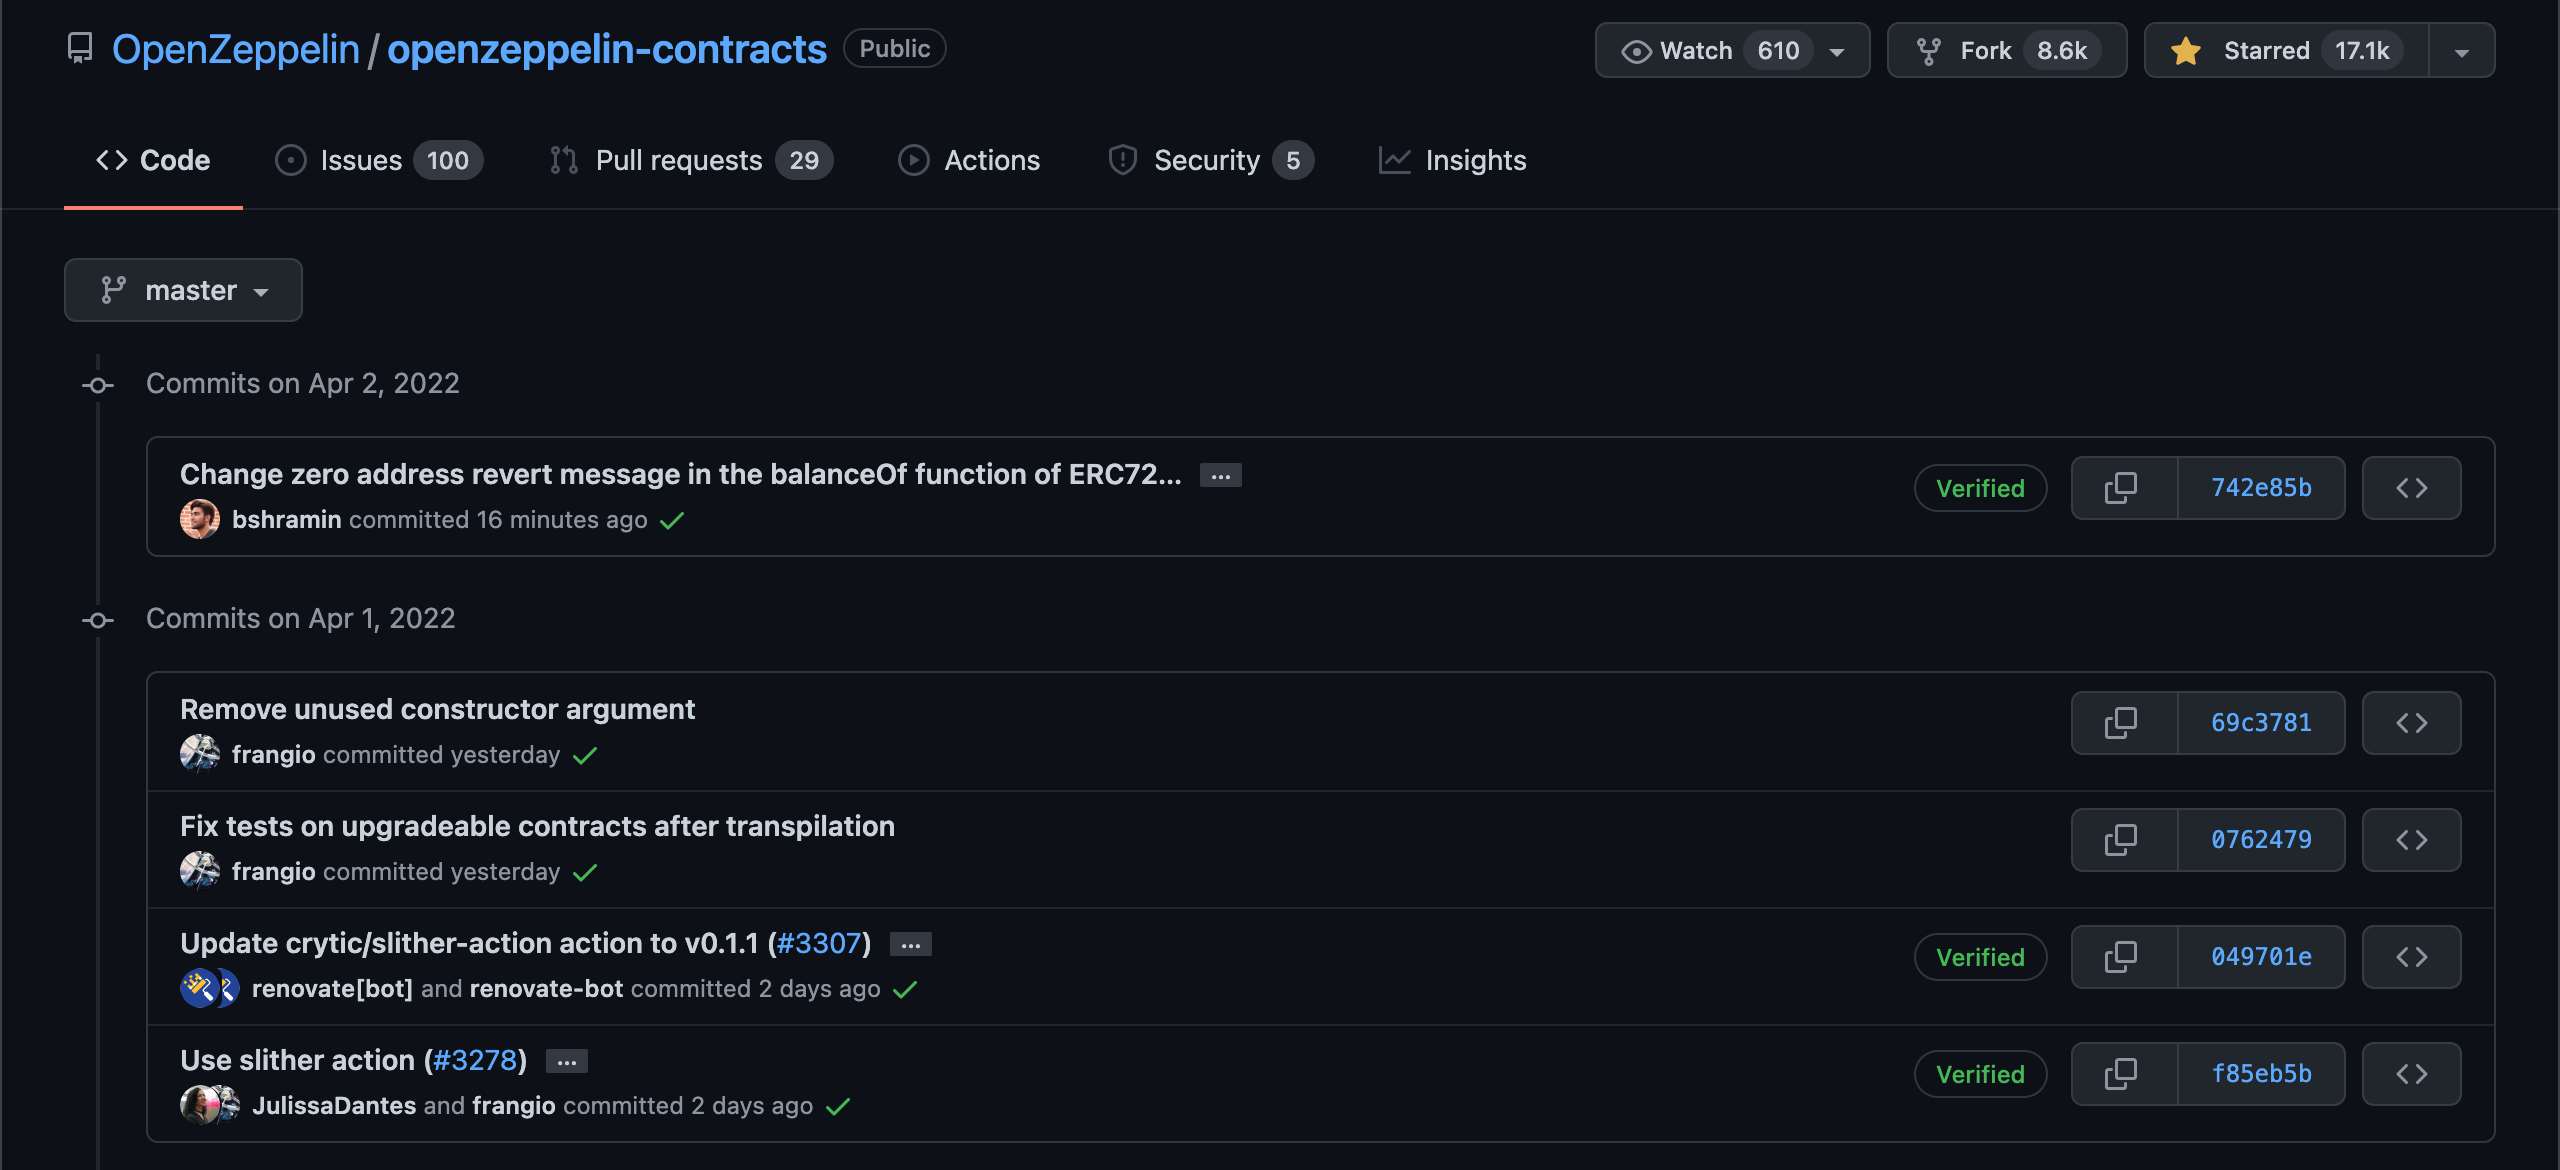
\includegraphics[width=15cm]{OpenZepplinContribution.png}}
\caption{در طی انجام پروژه مرج ریکوئستی روی OpenZeppelin باز شد که در همان روز مرج شد.}
\label{fig:zeppelin-merge-req}
\end{figure}


% ------------ Section 2.2
\section{آشنایی با مفهوم توکن تعویض ناپذیر}
شروع رمزارزها با توکن‌های تعویض پذیر بود، مفهوم تعویض پذیری به این معنی است که یک توکن با توکن دیگر تفاوتی ندارد و با جابه‌جا شدن آن‌ها تغییری ایجاد نمی‌شود. برای مثال یک بیت‌کوین با یک بیت‌کوین دیگر هیچ تفاوتی ندارد.

اما توکن‌های تعویض ناپذیر اینگونه نیستند، هر یک منحصر به فرد است و جابه‌جا کردن آن‌ها با یکدیگر تغییر ایجاد می‌کند،‌ در دنیای واقعی خانه می‌تواند مثال خوبی از یک دارایی تعویض ناپذیر باشد، هیچ دو خانه‌ای دقیقا شبیه به هم، در یک مکان، در طبقه یکسان و دارای پلاک مشترک نیستند.

پس مثلا به عنوان یک کاربرد، شهرداری می‌تواند یک قرارداد هوشمند ایجاد کند و به هر خانه یک توکن NFT اختصاص دهد. به این صورت صاحب خانه به جای سند یک توکن NFT دارد که مشخص می‌کند که دارایی متعلق به اوست، و فروش خانه به راحتی انتقال آن NFT به شخص دیگری است.

از نظر فنی هر توکن به این صورت یکتاست که یک \lr{Token ID} یکتا در قراردادش دارد و هر قرارداد هم دارای یک آدرس یکتا در شبکه بلاکچین است. پس ترکیب Contract Address و \lr{Token ID} باعث می‌شود که هر توکن یکتا باشد.


% ------------ Section 2.3
\section{کاربردها، حال و آینده}
کاربرد NFTها تا به حال در دو دسته خلاصه می‌شود. دسته اول به عنوان صاحب یک اثر دیجیتال، مانند یک تصویر یا یک موسیقی. دسته دوم به عنوان یک جواز یا بلیت برای ورود به جایی یا دریافت چیزی، برای مثال همایشی برگزار می‌شود که فقط دارندگان NFTهای یک قرارداد هوشمند می‌توانند به آن وارد شوند.

معروف‌ترین پلتفرم معاملاتی این توکن‌ها OpenSea است که می‌توان در آن توکن‌های موجود را مشاهده کرد و یک توکن را توسط مزایده خرید یا به فروش گذاشت. OpenSea در حال حاضر از قراردادهای شبکه‌های اتریوم و سولانا پشتیبانی می‌کند. دیگر شبکه‌ها نیز معمولا پلتفرم‌های خود را دارند، مانند شبکه Atom که در آن از پلتفرم Stargaze برای معامله NFTها استفاده می‌شود.

کاربردهای NFT ها در آینده می‌تواند بسیار وسیع باشد. دارایی‌های فیزیکی دنیای واقعی، بلیت‌های ورود به یک مکان یا یک همایش، دارایی‌های دنیای مجازی مانند یک موسیقی یا آیتمی در یک بازی و حتی دامنه‌های اینترنتی همه می‌توانند به NFT تبدیل شوند. مزایای تبدیل این موارد به NFT قابلیت نگهداری آسان‌تر، قابلیت فروش و انتقال راحت‌تر، امنیت بیشتر، آزادی در تراکنش‌ها و آشکار بودن مالکیت دارایی بر همگان است.


% ------------ Section 2.4
\section{قرارداد‌های هوشمند و استانداردسازی}
اکثر قرارداد‌های هوشمند قابلیت‌هایی مشابه با یکدیگر دارند، برای مثال گروهی از قرارداد‌های هوشمند توکن‌های تعویض پذیر دارند و گروه توکن‌های تعویض ناپذیر. از طرفی اپلیکیشن‌هایی مانند کیف‌پول‌های دیجیتال، پلتفرم‌های معاملاتی و صرافی‌های نیاز دارند که بتوانند دارایی‌های کاربر اعم از توکن‌های تعویض پذیر و تعویض ناپذیر را ببینند، به همین دلیل باید نحوه صحبت کردن با قراردادهای هوشمند را بدانند.

برای ساده‌تر کردن این فرایند و همسان‌سازی اینترفیس  این قراردادهای هوشمند استانداردهایی تعریف شده است که با استفاده از این استانداردها هم فرایند توسعه اسمارت کانترکت آسان‌تر خواهد شد و هم ارتباط میان قراردادهوشمند و اپلیکیشن‌های دیگر مانند کیف‌پول‌ها، پلتفرم‌های معاملاتی و ... آسان‌تر خواهد شد.

از نمونه‌های معروف این استانداردها
\lr{ERC20}
برای قرارداد‌هایی با توکن‌های تعویض پذیر و
\lr{ERC721}
برای قراردادهایی با توکن‌های تعویض ناپذیر است. در این پروژه از استاندارد
\lr{ERC721}
استفاده می‌شود اما در مورد
\lr{ERC1155}
هم مطالعه شده و توضیح داده می‌شود، به طور خلاصه
\lr{ERC1155}
قابلیت‌های بیشتری از
\lr{ERC721}
دارد و یک قرارداد با این استاندارد می‌تواند هم توکن‌های تعویض پذیر و هم تعویض ناپذیر داشته باشد.

برای استفاده از این استاندارد‌ها از پکیج‌های متن بازی استفاده می‌شود که این استاندارد‌ها را پیاده‌سازی کرده‌اند و از آن‌ها در قراردادی که نوشته می‌شود ارث‌بری می‌شود، یکی از بهترین پیاده‌سازی‌های این استاندارد‌های توسط
\gls{OpenZeppelin}
انجام شده است که در این پروژه نیز از همین پیاده‌سازی استفاده می‌شود.

\subsection{استاندارد \lr{ERC20}}
این استاندارد مناسب توکن‌های تعویض پذیر است. اینترفیسی تعریف می‌کند که نیازهای قراردادهایی با توکن‌های تعویض پذیر را برطرف کند و نحوه تعامل برقرار کردن با آن‌ها را یکسان گرداند. در این استاندارد فقط می‌توان یک نوع توکن تعویض پذیر به تعداد دلخواه داشت. این استاندارد متدهایی برای تعریف حداکثر تعداد توکن‌های موجود، گرفتن موجودی یک آدرس، و انتقال توکن‌ها دارد. توضیحات دقیق‌تر در مورد این استاندارد را می‌توان در وبسایت
اتریوم
\LTRfootnote{\url{https://ethereum.org/en/developers/docs/standards/tokens/erc-20}}
یا اپن‌زپلین
\LTRfootnote{\url{https://docs.openzeppelin.com/contracts/4.x/api/token/erc20}}
مشاهده کرد.

\subsection{استاندارد \lr{ERC721}}
استفاده از استاندارد
\lr{ERC721}
برای توکن‌های تعویض ناپذیر بسیار مرسوم است. در این استاندارد متدها و ایونت‌هایی برای یکسان سازی اینترفیس قراردادهای دارای توکن‌های تعویض ناپذیر تعریف شده است. در این نوع قرارداد‌ها می‌توان به تعداد دلخواه توکن‌های متفاوت با یکدیگر داشت، هر توکن یک شناسه یکتا دارد که می‌تواند به صورت ترتیبی یا غیر ترتیبی ایجاد شود.

همچنین متدی وجود دارد که می‌تواند شناسه یک توکن را به آدرسی تبدیل کند که اطلاعات آن توکن در آنجا موجود است. کاربرها می‌توانند توکن‌هایی که دارند را مشاهده کنند، به یکدیگر ارسال کنند یا به آدرس دیگری وکالت بدهند که توکن‌ها را به شخص دیگری ارسال کند.

تنها قابلیتی که به طور مشخص در این قرارداد معین نشده است که چگونه باید انجام شود قابلیت
\gls{Mint}
توکن‌ها است. اکثر قراردادهای هوشمندی که توکن‌های تعویض ناپذیر دارند به کاربران اجازه ساخت توکن‌ها را نمی‌دهند و ساخت توکن‌ها فقط به آدرس صاحب قرارداد محدود می‌شود. اما در کاپو اینگونه نیست و هرکسی می‌تواند برای خودش توکن بسازد.

اطلاعات دقیق‌تر در مورد این استاندارد را نیز می‌توان در وبسایت
اتریوم
\LTRfootnote{\url{https://ethereum.org/en/developers/docs/standards/tokens/erc-721}}
یا
اپن‌زپلین
\LTRfootnote{\url{https://docs.openzeppelin.com/contracts/4.x/api/token/erc721}}
مشاهده کرد.


\subsection{استاندارد \lr{ERC1155}}
تا اینجا با معروف‌ترین استاندارد‌های موجود برای قراردادهایی که توکن‌های تعویض پذیر یا تعویض ناپذیر دارند آشنا شدیم. اما همچنان نیازمندی‌هایی وجود دارند که توسط هیچ‌یک از این استانداردها برطرف نمی‌شوند. نیازمندی‌هایی مانند:
\begin{itemize}
	\item
داشتن توکن‌های NFT با تعداد محدود به جای فقط یکی.
	\item
داشتن همزمان چندین نوع توکن مختلف در یک قرارداد.
	\item
انتقال همزمان چند توکن از انواع مختلف از کاربری به کاربر دیگر.
\end{itemize}

یک مثال از کاربردی که به این قابلیت‌ها نیاز دارد می‌تواند یک بازی مثل مونوپولی باشد که در آن هر کاربر مقداری پول دارد که در واقع یک توکن تعویض پذیر هست، به عنوان دارایی چند خانه دارد که به عنوان توکن‌های تعویض ناپذیری هستند که از هرکدام فقط یکی وجود دارد و ممکن است چند کارت خروج از زندان داشته باشد که یکتا نیستند اما تعداد محدودی در بازی وجود دارد. استاندارد
\lr{ERC1155}
همه‌ی این نیازها را برطرف می‌کند. همه‌ی این چند نوع توکن می‌توانند همزمان در یک قرارداد هوشمند وجود داشته باشند.

در این استاندارد متدهایی برای تعریف نوعی توکن با تعداد مشخص وجود دارد. اگر نیاز به توکنی تعویض ناپذیر باشد تعداد آن یک قرارداده می‌شود. همچنین متدهایی برای ارسال تعداد مشخص از چند نوع توکن مختلف در یک تراکنش، دادن وکالت توکن‌ها به آدرس دیگر و گرفتن موجودی یک آدرس در این استاندارد وجود دارد.

اطلاعات دقیق‌تر در مورد این استاندارد را نیز می‌توان در وبسایت
اتریوم
\LTRfootnote{\url{https://ethereum.org/en/developers/docs/standards/tokens/erc-1155}}
یا
اپن‌زپلین
\LTRfootnote{\url{https://docs.openzeppelin.com/contracts/4.x/api/token/erc1155}}
مشاهده کرد.
		% فصول دوم: مروری بر مطالعات انجام شده
% !TeX root=../main.tex
\chapter{آشنایی با ابزار‌های توسعه}
در تمام ابزارهای ذکر شده در ادامه این متن حتما باید به ورژن هر کدام دقت شود، ورژن‌ها باید با یکدیگر همخوانی داشته باشند در غیر این صورت مشکلاتی در کامپایل و اجرای برنامه به وجود می‌آید که به راحتی قابل رفع کردن نیستند. در انجام این پروژه عدم همخوانی ورژن‌های مختلف ابزارها با یکدیگر باعث ایجاد مشکلات فراوانی شد، به همین دلیل ورژن مورد نیاز هر ابزار در توضیحات پروژه ذکر شده است.

% ------------ Section 2.1
\section{ابزارهای ساده}
\begin{itemize}
	\item \textbf{ویرایشگر}\\
	برای برنامه نویسی این قرارداد هوشمند از ویرایشگر VSCode با نصب
	پلاگین مربوط به Solidity
\LTRfootnote{https://marketplace.visualstudio.com/items?itemName=JuanBlanco.solidity}
استفاده شده است. این پلاگین با یافتن اشتباه‌ها پیش از کامپایل و راهنمایی در نوشتن کد قرارداد کمک شایانی به افزایش سرعت توسعه می‌کند.

	\item \textbf{ورژن‌کنترل}\\
	این پروژه از روز نخست به صورت متن‌باز توسعه یافته، برای توسعه یک پروژه به صورت متن‌باز اولین ابزار مورد نیاز یک برنامه ورژن کنترل است که نسخه‌های متفاوت و تغییر یافته کدها را به صورت مرتب نگهداری کند. برای این منظور از گیت‌هاب استفاده شده.

	\item \textbf{پکیج‌های Node و NPM}\\
از آنجایی که کدهای سالیدیتی در واقع جاوا‌اسکریپت هستند، به ابزارهای توسعه اپلیکیشن‌های جاوااسکریپت برای توسعه سالیدیتی نیاز است. ابزارهایی مانند Node برای کامپایل کردن برنامه‌های جاوااسکریپت و npm که مدیریت پکیج‌های جاوااسکریپتی که نصب می‌شود را به عهده دارد.

\end{itemize}


		% فصل سوم: روش تحقیق
% !TeX root=../main.tex
\chapter{پیاده‌سازی}

% ------------ Section 4.1
\section{نوشتن کد قرارداد}
در این بخش به بررسی مراحل و نحوه نوشتن کد قراردادهوشمند پرداخته می‌شود.

% ------------ Sub Section 4.1.1
\subsection{نیازمندی‌های قراردادهوشمند}
نیازمندی‌های اصلی کاپو به ترتیب زیر است.
\begin{itemize}
  \item
هر آدرس در شبکه بتواند یک داده‌ی متنی را به آسان‌ترین و کم هزینه‌ترین روش ممکن به یک توکن NFT تبدیل کند.
  \item
هر آدرس بتواند توکن‌های خود را به اشخاص دیگر انتقال دهد یا در بازارهای معاملات NFT بفروشد.
  \item
در صفحه اول وبسایت تعداد کل توکن‌های ساخته شده تا به حال و تعداد کل دارندگان توکن نمایش داده شود.
  \item
قابلیت‌های قراردادهوشمند تست شده باشد.
\end{itemize}

% ------------ Sub Section 4.1.2
\subsection{ارث‌بری}
با توجه به مزایای ذکر شده در مورد استانداردسازی قراردادهای هوشمند، انتخاب درستی است که برای پیاده‌سازی این کاربری از یکی از استانداردها استفاده شود. ارثبری از استانداردهای یک کتابخانه متن‌باز مزایای زیر را فراهم می‌کند.
\begin{itemize}
  \item
به دلیل وجود کدهای پایه به صورت آماده سرعت توسعه پروژه افزایش می‌یابد.
  \item
ارتباط دیگر پروژه‌ها با پروژه کاپو به راحتی انجام می‌شود.
  \item
امنیت قرارداد و درستی آن حداقل در سطوح پایه‌ای تا حد خوبی تضمین شده است.
\end{itemize}

قراردادهوشمند کاپو از استاندارد ERC721 پیاده‌سازی شده در کتابخانه اپن‌زپلین
\LTRfootnote{
  \url{https://github.com/OpenZeppelin/openzeppelin-contracts}
}
ارث‌بری می‌کند که یکی از معروف ترین کتابخانه‌های پیاده کننده استانداردهای قرارداد هوشمند است.

% ------------ Sub Section 4.1.3
\subsection{توجه به هزینه تراکنش و نوع توابع}
در نوشتن یک قراردادهوشمند باید به نکات زیر توجه کنیم.
\begin{itemize}
  \item
میزان حافظه‌ای که اشغال می‌کنیم.
  \item
حجم بایت‌کد.
  \item
میزان عملیات هر متد، به خصوص متدهایی که مکررا مورد استفاده کاربر قرار می‌گیرند.
  \item
نوع هر متد، که مشخص می‌کند هر متد تا چه حد روی شبکه بلاکچین تغییر ایجاد می‌کند.
\end{itemize}

توجه نکردن به هریک از این موضوعات باعث می‌شود که قراردادهوشمند به اندازه کافی بهینه عمل نکند و کاربر وادار به پرداخت gas fee یا هزینه تراکنش بیشتر شود. یکی از مهمترین نکاتی که برای بهینه‌تر رفتار کردن قراردادهوشمند باید به آن توجه کنیم نوع هر متد است.

اگر متدی از نوع pure تعریف شود به این معنی است که به هیچ اطلاعاتی از شبکه بلاک‌چین نیاز ندارد و همه‌ی اطلاعاتی که لازم دارد را در اسکوپ
\LTRfootnote{Scope}
خودش دارد. اگر متدی از نوع view باشد به این معنی است که به اطلاعاتش روی شبکه بلاکچین نیاز دارد اما فقط می‌خواهد که آن‌ها را بخواند و نمیخواهد تغییری در آن‌ها ایجاد کند. این دو نوع متد نیازی به پرداخت کارمزد تراکنش توسط کاربر ندارند، اما اگر در تعریف متدی ذکر نشود که یکی از این دو نوع است، اینطور در نظر گرفته می‌شود که نیاز به بروزرسانی اطلاعاتش در شبکه بلاکچین دارد و از کاربری که آن را فراخوانی کرده است هزینه تراکنش دریافت می‌شود.


% ------------ Sub Section 4.1.4
\subsection{جزئیات فنی پیاده‌سازی}
مینت کردن در این قرارداد به آدرس‌های مشخص محدود نیست و همه می‌توانند توکن بسازند. بسیاری از قراردادها برای صرفه‌جویی در هزینه تراکنش کاربران اکثر اطلاعات مربوط به توکن‌ها را در قرارداد نگه نمیدارند و فقط داده‌های بسیار مهم توکن را در شبکه بلاکچین نگهداری می کنند. از آنجایی که کاپو یک قرارداد همه منظوره است و ممکن است استفاده‌های فراوانی داشته باشد، تصمیم‌گیری این مورد به عهده کاربر قرارداد گذاشته می‌شود.

در کاپو آیدی هر توکن از hash داده‌های توکن به دست می‌آید. این نحوه عملکرد چند مزیت ایجاد می‌کند. به این ترتیب هیچ دو توکنی نمی‌توانند داده‌های یکسان داشته باشند، زیرا در این صورت آیدی آن‌ها باید یکسان باشد و این امکان پذیر نیست زیرا آیدی توکن‌ها یکتاست. همچنین آیدی توکن‌ها دیگر ترتیبی نخواهند بود و ترتیب ساخت توکن‌ها مشخص نخواهد بود.

در یک قرارداد ERC721 استاندارد فقط آیدی توکن‌ها ذخیره می‌شود. در کاپو علاوه بر آیدی توکن‌ها یک map از آیدی توکن‌ها به داده‌ی آن‌ها با نام tokenDatas نیز نگهداری می‌شود. همچنین در کاپو map دیگری نیز از آدرس به لیست توکن‌های آن آدرس با نام ownerTokens نگهداری می‌شود. متغیر اول کمک می‌کند که با داشتن آیدی یک توکن به راحتی داده‌های آن توکن به دست آورده شوند. متغیر دوم نیز کمک می‌کند که به راحتی بتوان توکن‌های یک آدرس را به دست آورد. دو متغیر دیگر با نام‌های numberOfTokenHolders و numberOfMintedTokens نیز در کاپو نگه‌داشته می‌شوند که برای نمایش آمار استفاده از قرارداد در صفحه اصلی اپلیکیشن مورد استفاده قرار می‌گیرند.

متد mint به نحوی نوشته شده است که برای عموم قابل استفاده باشد. پس از محاسبه hash داده‌ی توکن از آن به عنوان آیدی توکن استفاده می‌کند، توکن را می‌سازد و متغیرهای tokenDatas و numberOfMintedTokens را بروزرسانی می‌کند.

\begin{figure}[ht]
\centerline{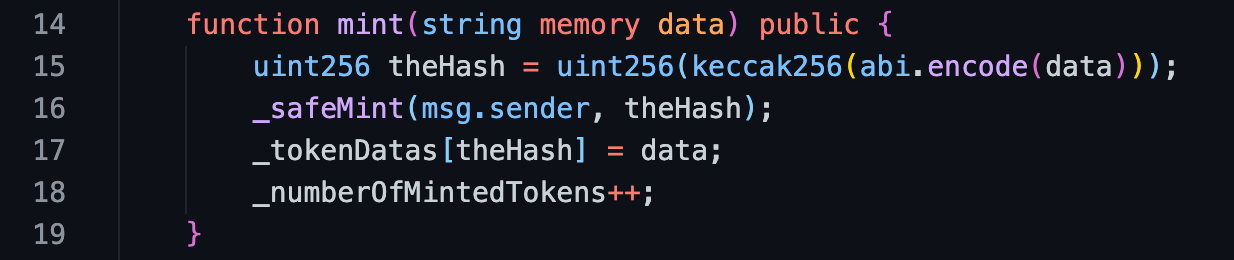
\includegraphics[width=12cm]{mint.png}}
\caption{پیاده‌سازی تابع mint}
\label{fig:mint}
\end{figure}

متد afterTokenTransfer از استاندارد ERC721 به نحوی بازنویسی
\LTRfootnote{Overwrite}
شده است که پس از هر انتقال توکن با بررسی آدرس‌های مبدا و مقصد، متغیر‌های numberOfTokenHolders و numberOfMintedTokens و ownerTokens را بروزرسانی کند.

\begin{figure}[ht]
\centerline{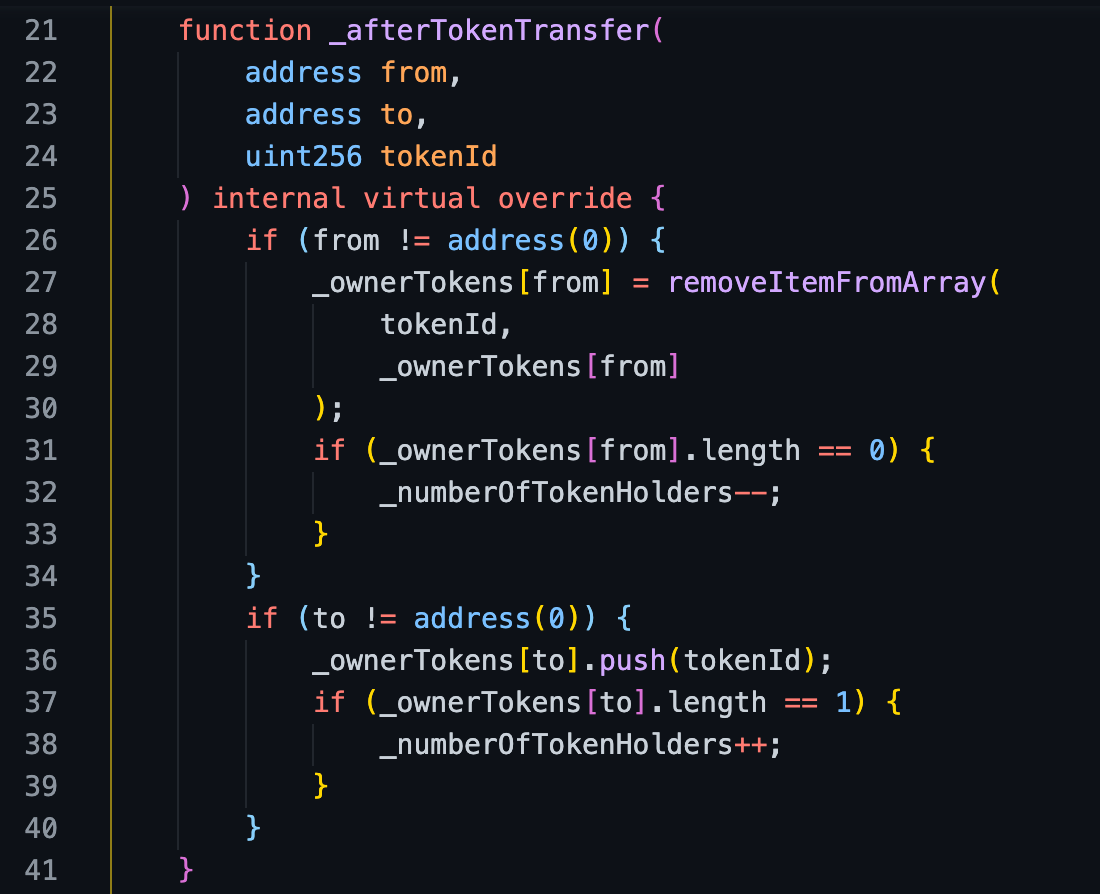
\includegraphics[width=12cm]{afterTokenTransfer.png}}
\caption{پیاده‌سازی تابع afterTokenTransfer}
\label{fig:afterTokenTransfer}
\end{figure}

متد جدیدی با نام getUserTokens نیز نوشته شده است که در استاندارد ERC721 به صورت پیش‌فرض وجود ندارد. این متد با گرفتن یک آدرس و استفاده از ownerTokens و tokenDatas دو خروجی برمی‌گرداند، لیستی از آیدی توکن‌های آدرس و لیستی از داده‌های توکن‌های آدرس.

\begin{figure}[ht]
\centerline{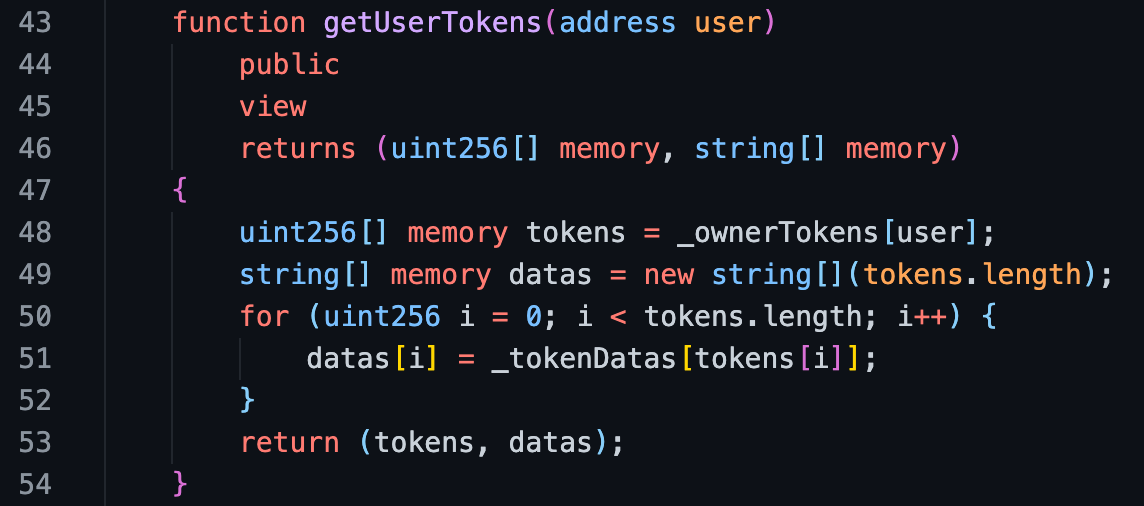
\includegraphics[width=12cm]{getUserTokens.png}}
\caption{پیاده‌سازی تابع getUserTokens}
\label{fig:getUserTokens}
\end{figure}

همچنین از آنجایی که سالیدیتی به طور پیش‌فرض امکان حذف یک داده از یک آرایه با داشتن مقدار آن را ندارد، عدم وجود این قابلیت هزینه‌بر بودن آن است، در سالیدیتی توسعه دهندگان به استفاده از map و دوری از array ها تشویق می‌شوند. اما برای نمایش نحوه ارث‌بری از دو یا چند قرارداد پدر، برای کاپو یک قرارداد به نام Helper نوشته شد که این قابلیت را فراهم می‌کند. کاپو علاوه بر
\lr{ERC721}
از قرارداد Helper نیز ارث‌بری می‌کند.

\begin{figure}[ht]
\centerline{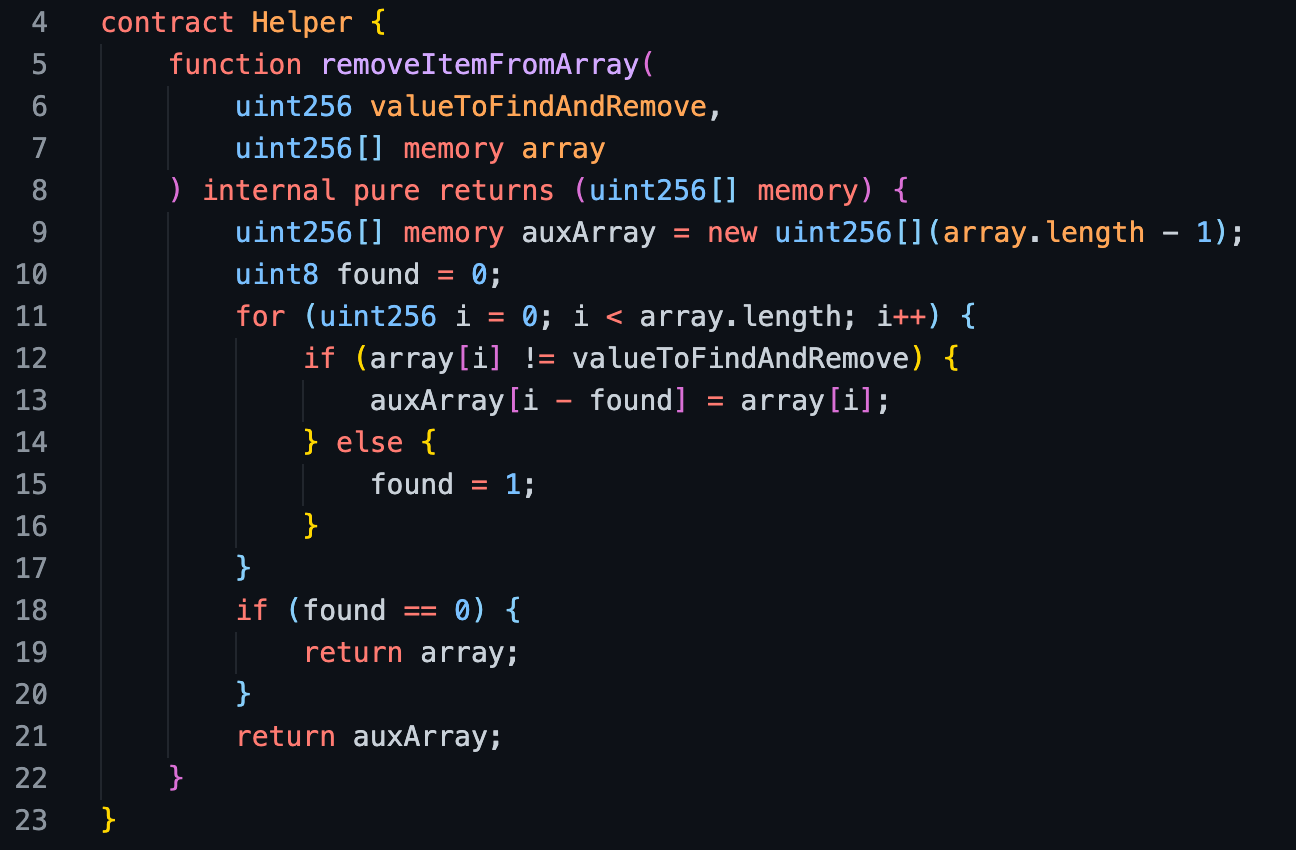
\includegraphics[width=12cm]{Helper.png}}
\caption{پیاده‌سازی قرارداد Helper}
\label{fig:Helper}
\end{figure}

% ------------ Section 4.2
\section{نوشتن و اجرای تست‌ها}
پیش‌تر اشاره شد که از مزیت‌های ارث‌بری از کتابخانه‌های متن‌باز معروف این است که احتمال وجود خطا و مشکل امنیتی به شدت کمتر می‌شود. یکی از دلایل این مسئله این است که این کتابخانه‌ها پوشش تستی به شدت بالایی دارند. به همین دلیل می‌توان تا حدی به عملکرد قرارداد پدر اطمینان خاطر داشت و بیشتر روی تست کردن قابلیت‌های اضافه شده در قراردادهوشمند فرزند تمرکز داشت.

در کاپو برای هر عملکرد قرارداد تست نوشته شده است. یکی از ساده‌ترین تست‌های نوشته شده تست فرآیند ساخت یک توکن است که در آن پس از دیپلوی قرارداد با فراخوانی متد mint یک توکن ساخته می‌شود و سپس با فراخوانی متد balanceOf دارایی آدرس سازنده توکن بررسی می‌شود و انتظار می‌رود که پس از ساخت یک توکن، دارایی آدرس سازنده توکن یک باشد. این تست را می‌توان در تصویر زیر مشاهده کرد.

\begin{figure}[ht]
\centerline{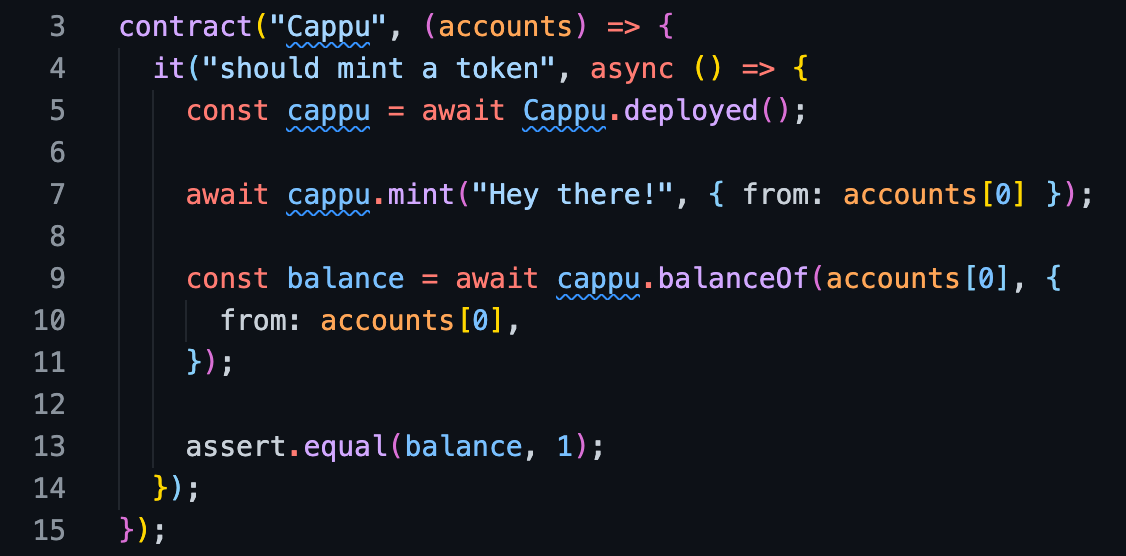
\includegraphics[width=12cm]{mint-test.png}}
\caption{نمونه یکی از تست‌های قرارداد کاپو}
\label{fig:mint-test}
\end{figure}

پس از نوشته شدن تست‌ها می‌توان آن‌ها را با اجرای دستور
\lr{truffle test}
اجرا کرد. این دستور پس از اجرای تست‌ها نتیجه و زمان اجرای هر تست را به عنوان خروجی نمایش می‌دهد. نمونه اجرای این دستور را می‌توان در تصویر زیر مشاهده کرد.

\begin{figure}[ht]
\centerline{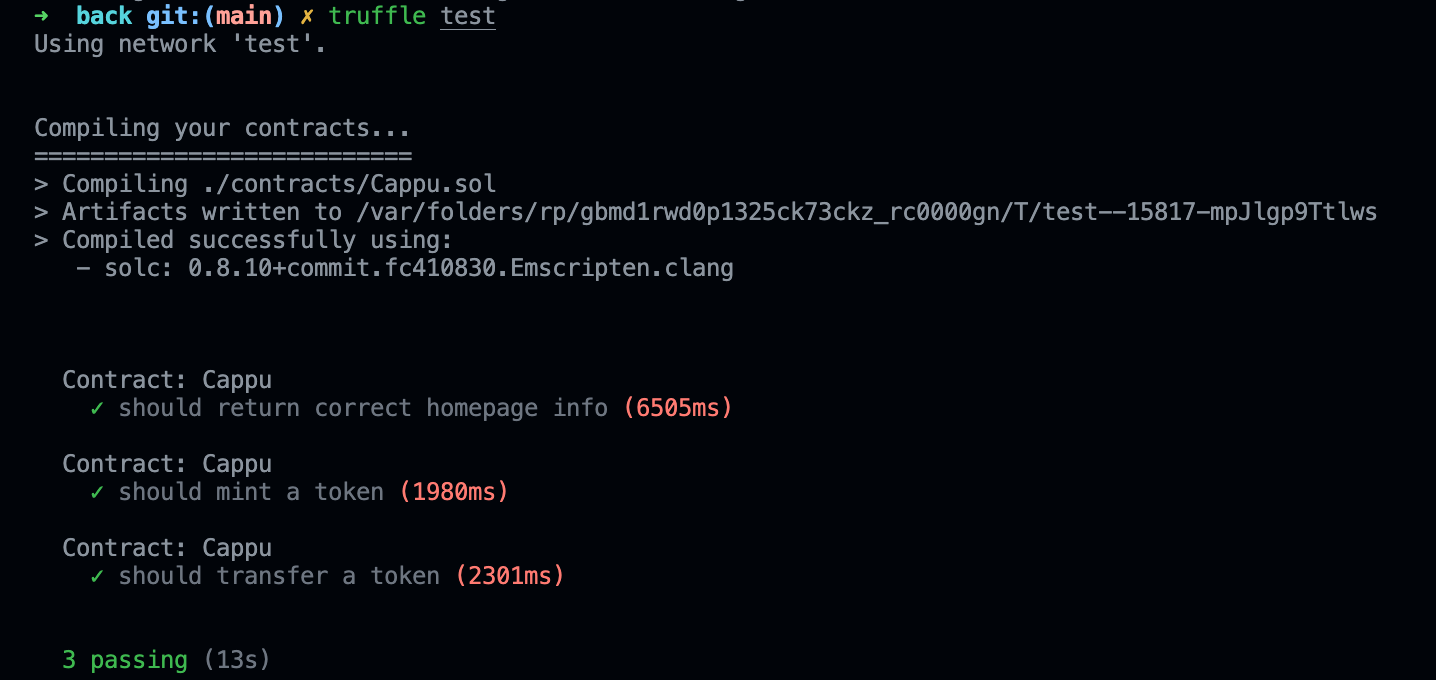
\includegraphics[width=12cm]{test-output.png}}
\caption{نمونه خروجی اجرای تست‌های قرارداد}
\label{fig:test-output}
\end{figure}

% ------------ Section 4.3
\section{دیپلوی قرارداد روی شبکه تستی Ropsten}
تا اینجا قراردادهوشمند نوشته و تست شده است، در این مرحله روی شبکه تستی Ropsten دیپلوی می‌شود. فرآیند دیپلوی شدن کاپو به کمک چارچوب ترافل قدم به قدم شرح داده می‌شود.

\subsection{یافتن آدرس یکی از نود‌های شبکه برای ارسال تراکنش دیپلوی قرارداد به آن}
آدرس نود‌های یک شبکه بلاکچین همه به صورت عمومی در دسترس هستند زیرا نودها باید بتوانند یکدیگر را ببینند. راه‌های زیادی برای به دست آوردن آدرس یک نود وجود دارد. یکی از آسان‌ترین راه‌های به دست آوردن آدرس یکی از نود‌های شبکه مراجعه به وبسایت ماینر است. برای این پروژه از وبسایت Moralis
\LTRfootnote{
  \url{https://moralis.io}
}
برای پیدا کردن آدرس نود شبکه استفاده شد.

\begin{figure}[ht]
\centerline{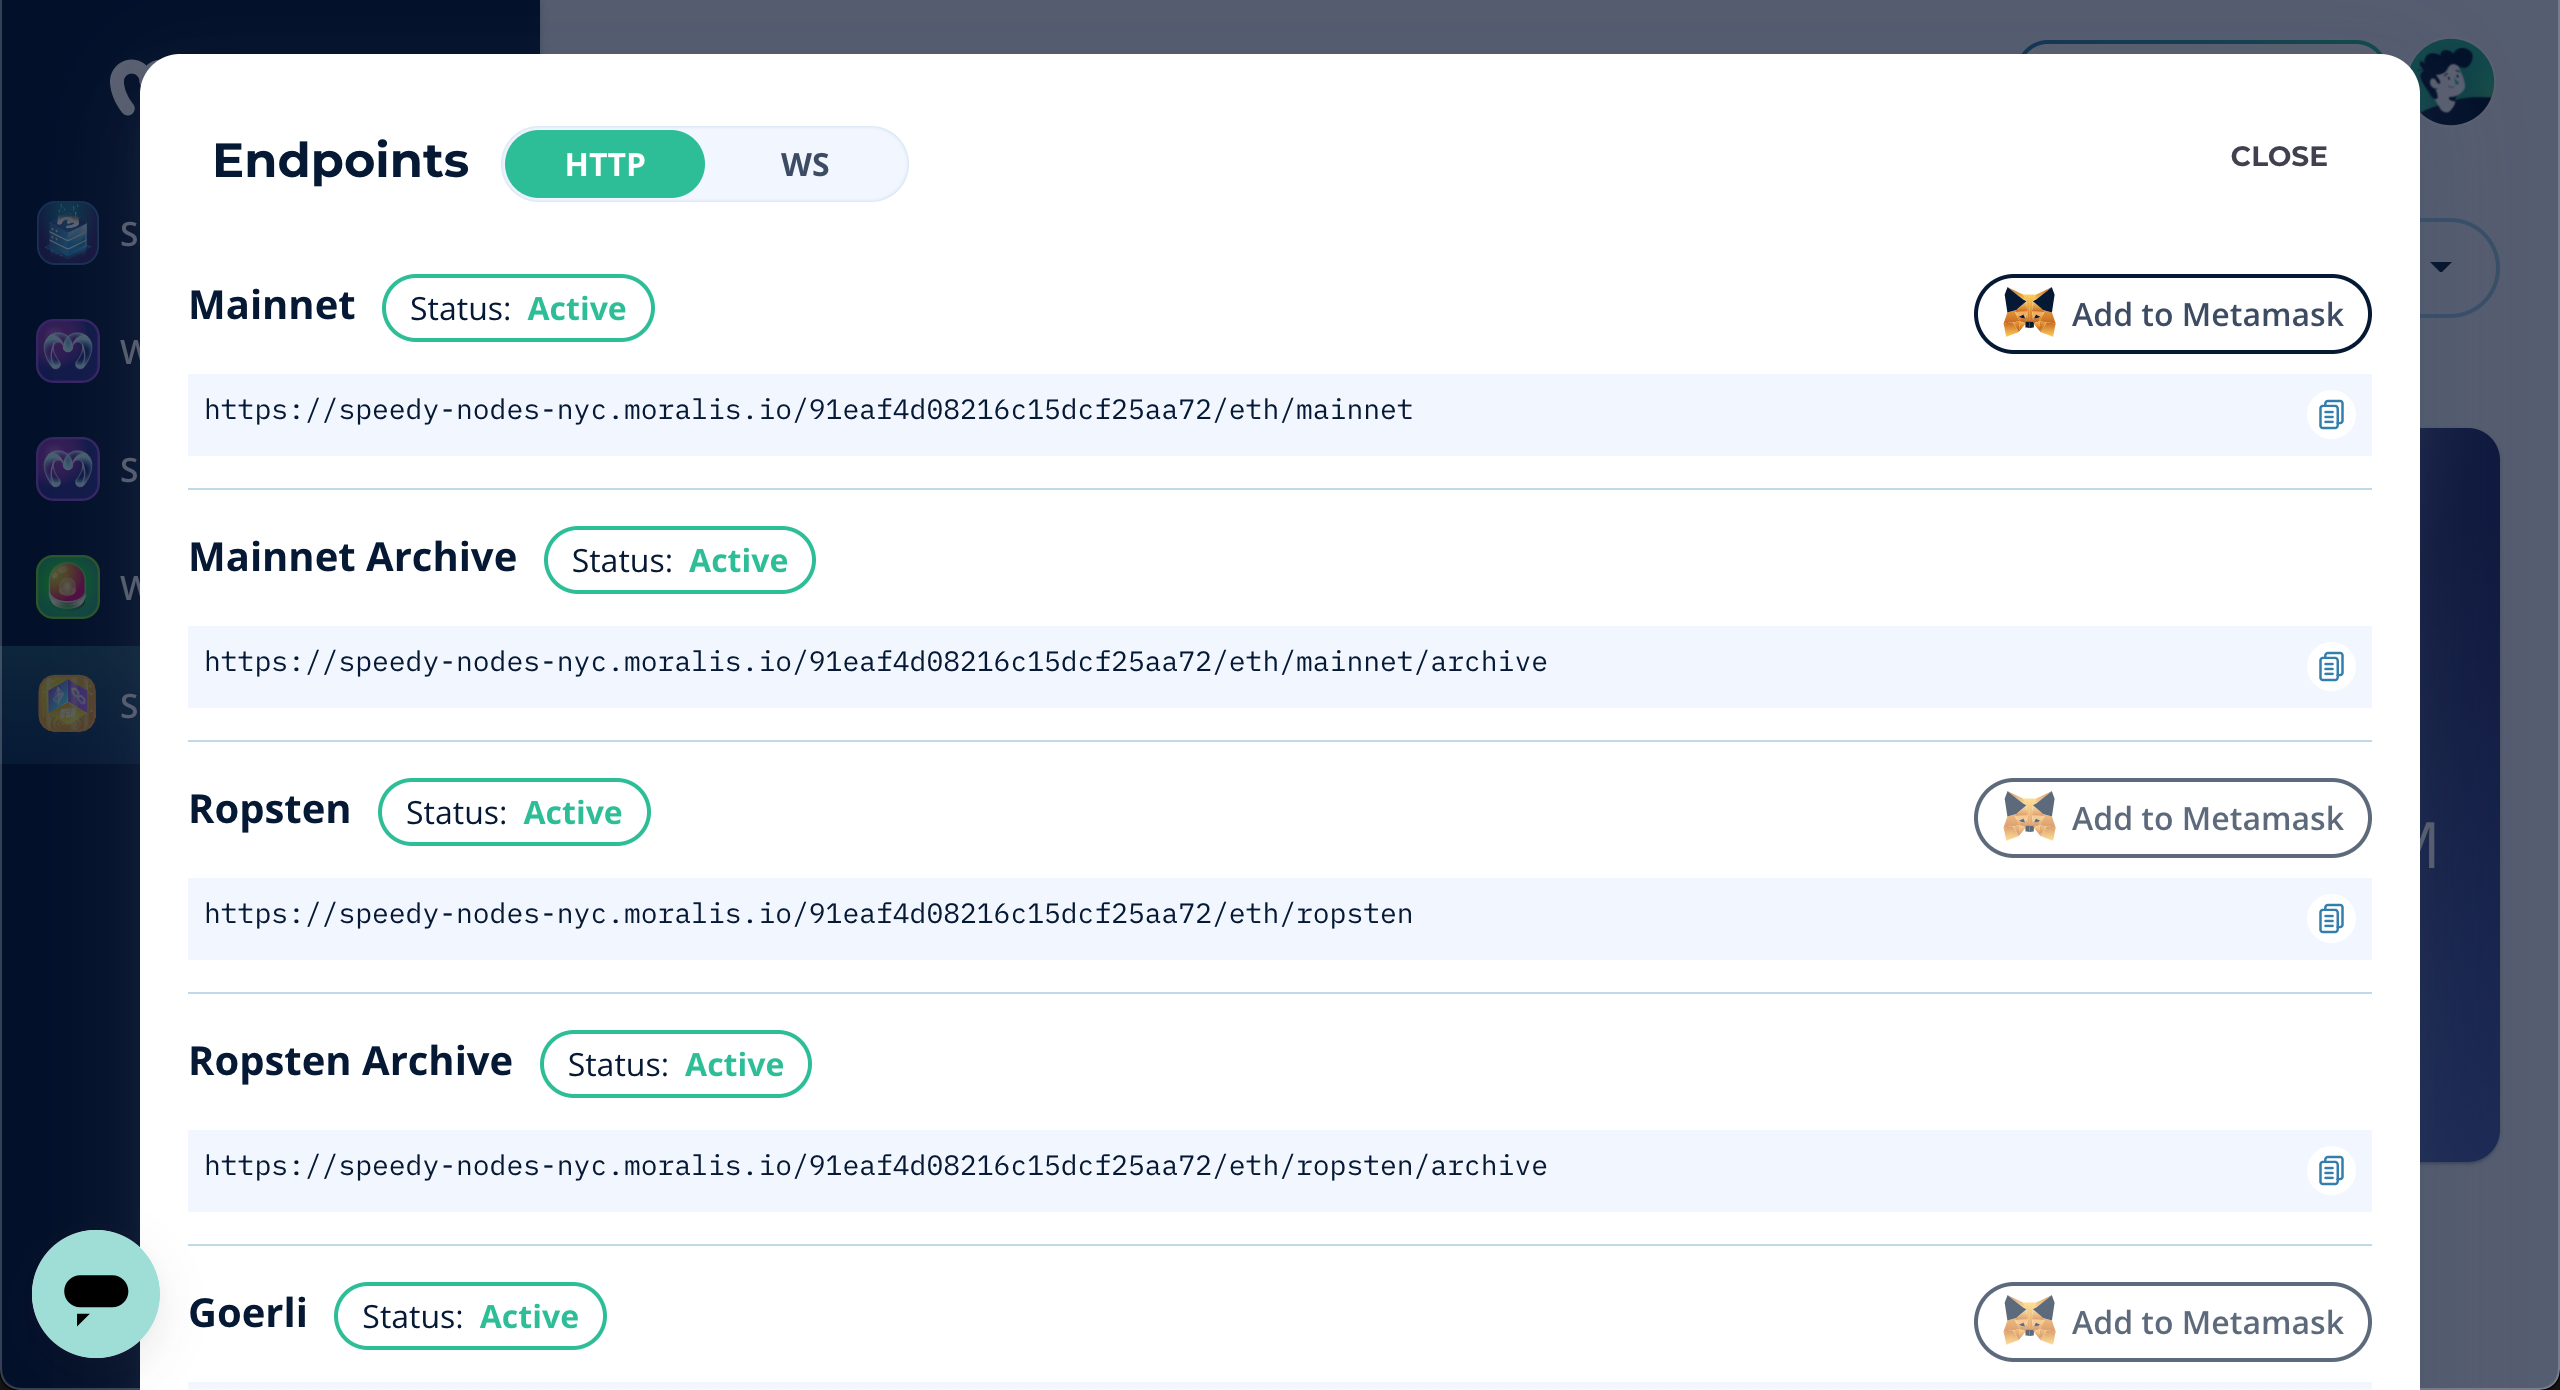
\includegraphics[width=12cm]{moralis.png}}
\caption{دریافت آدرس یکی از نود‌های شبکه از وبسایت Moralis}
\label{fig:moralis}
\end{figure}

\subsection{اضافه شدن اطلاعات شبکه مورد نظر به تنظیمات ترافل}
هنگامی که به کمک دستور
\lr{truffle init}
یک پروژه ترافل ساخته می‌شود، فایلی با نام truffle-config.js ساخته می‌شود. تنظیمات مربوط به ترافل در این فایل نوشته شده‌است. برای این که ترافل شبکه مورد نظر را بشناسد باید اطلاعات آن شبکه در این فایل نوشته و شبکه‌ی جدیدی تعریف شود. برای تعریف شبکه از آدرسی که در گام قبل به دست آمد استفاده می‌شود و مانند تصویر زیر شبکه‌ی جدیدی تعریف می‌شود.

\begin{figure}[ht]
\centerline{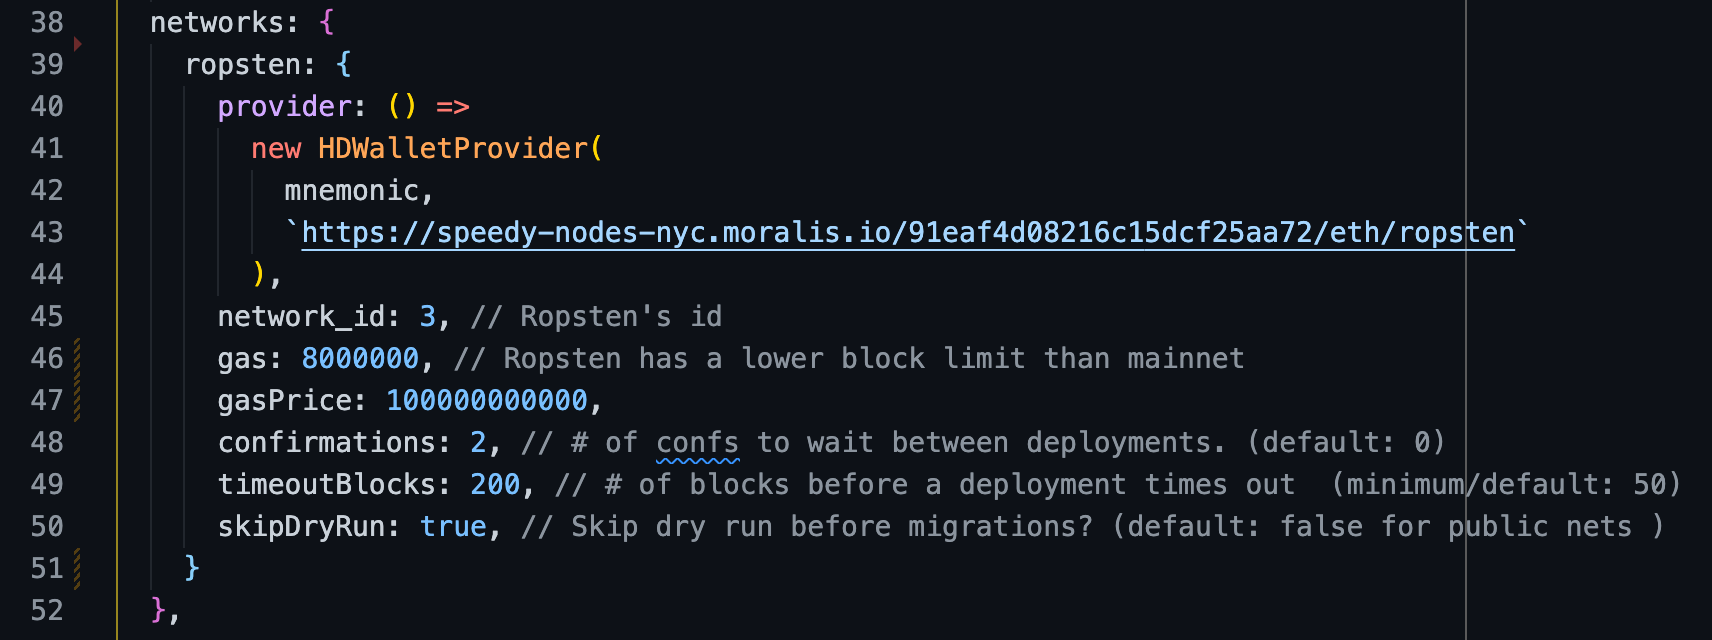
\includegraphics[width=12cm]{network-config.png}}
\caption{اضافه کردن شبکه Ropsten به شبکه‌های ترافل}
\label{fig:network-config}
\end{figure}


\subsection{آماده شدن mnemonics}
برای انجام این پروژه به کمک دستور
\lr{npm mnemonics}
یک آدرس تستی ساخته می‌شود. این دستور، mnemonics متناسب با این آدرس را به عنوان خروجی می‌دهد. دقت کنید که برای دیپلوی روی
\gls{Mainnet}
حتما باید از mnemonics مربوط به یک کیف پول واقعی استفاده شود و اطلاعات ان در اختیار کسی قرار نگیرد.

\begin{figure}[ht]
\centerline{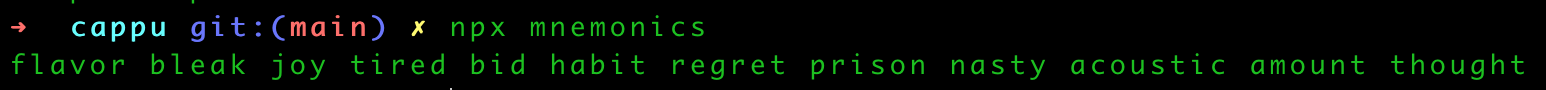
\includegraphics[width=12cm]{mnemonics.png}}
\caption{ایجاد mnemonics تستی}
\label{fig:mnemonics}
\end{figure}


\subsection{استفاده از کیف پول ایجاد شده در تنظیمات ترافل}
ترافل برای این که بتواند از کیف‌پول برای انجام تراکنش‌ها استفاده کند باید به mnemonics یا کلید خصوصی آن دسترسی داشته باشد. به این منظور فایلی با نام secrets.json در دایرکتوری اصلی برنامه ساخته می‌شود و mnemonics کیف پول به شکل زیر در آن قرار داده می‌شود.

\begin{figure}[ht]
\centerline{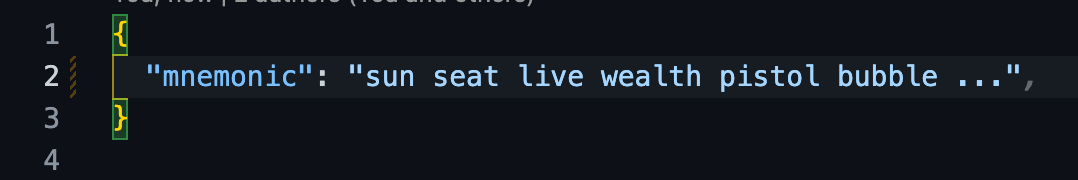
\includegraphics[width=12cm]{mnemonics-in-secrets.png}}
\caption{قراردادن mnemonics در فایل secrets.json}
\label{fig:mnemonics-in-secrets}
\end{figure}

سپس در تنظیمات ترافل باید ذکر شود که می‌تواند آدرس کیف‌پول را در این آدرس پیدا کند.

\begin{figure}[ht]
\centerline{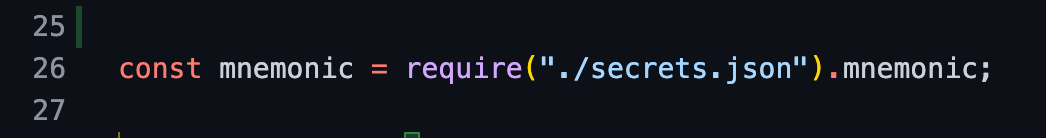
\includegraphics[width=12cm]{secrets-in-config.png}}
\caption{معرفی فایل secrets.json در تنظیمات ترافل}
\label{fig:secrets-in-config}
\end{figure}


\subsection{نصب کیف‌پول hdwallet}
ترافل برای استفاده از mnemonics کیف پول ما نیاز به نصب پکیج hdwallet-provider دارد، این پکیج کاربری‌های یک کیف پول دیجیتال از جمله امضا و ارسال تراکنش بر روی شبکه بلاکچین را در اختیار ترافل قرار می‌دهد. این پکیج با اجرای دستور
\lr{npm install –save-dev @truffle/hdwallet-provider}
نصب می‌شود.  پس از نصب کیف پول در تنظیمات ترافل در فایل truffle-config.js ذکر می‌شود که از این کیف‌پول استفاده شود.

\begin{figure}[ht]
\centerline{
\includegraphics[width=12cm]{wallet-in-config.png}}
\caption{استفاده از کیف‌پول hdwallet در تنظیمات ترافل}
\label{fig:wallet-in-config}
\end{figure}


\subsection{انتخاب شبکه اضافه شده}
حال هنگام ورود به خط فرمان ترافل مانند تصویر زیر شبکه مورد نظر انتخاب می‌شود.

\begin{figure}[ht]
\centerline{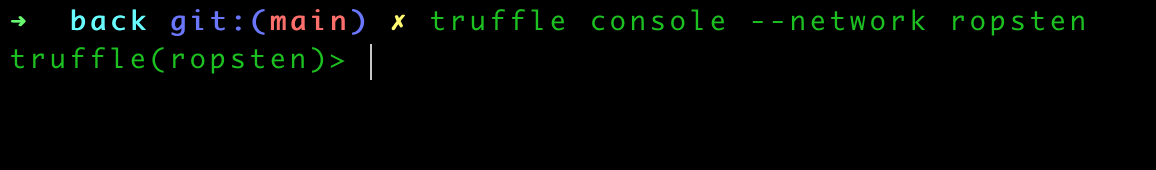
\includegraphics[width=12cm]{truffle-console.png}}
\caption{ورود به خط فرمان ترافل با انتخاب شبکه Ropsten}
\label{fig:truffle-console}
\end{figure}


\subsection{بررسی آدرس کیف‌پول و موجودی آن}
برای دیپلوی یک قرارداد هوشمند باید آدرس دیپلوی کننده آن بتواند هزینه تراکنش دیپلوی را پرداخت کند. در صورتی که دیپلوی بر روی یک شبکه تستی انجام می‌شود باید با استفاده از یک faucet روی شبکه تستی به میزان کافی پول تستی دریافت شود.

برای دریافت آدرس‌های کیف‌پول از دستور زیر در خط فرمان ترافل استفاده می شود.

\begin{figure}[ht]
\centerline{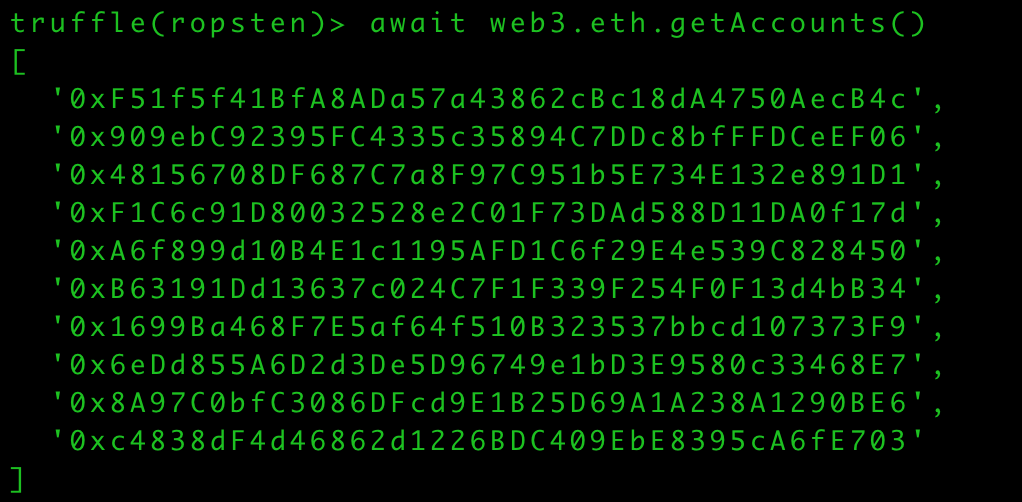
\includegraphics[width=12cm]{get-addresses.png}}
\caption{دریافت آدرس‌های کیف‌پول در خط فرمان ترافل}
\label{fig:get-addresses}
\end{figure}

برای دریافت مانده حساب آدرس، دستور زیر در خط فرمان ترافل اجرا می‌شود.

\begin{figure}[ht]
\centerline{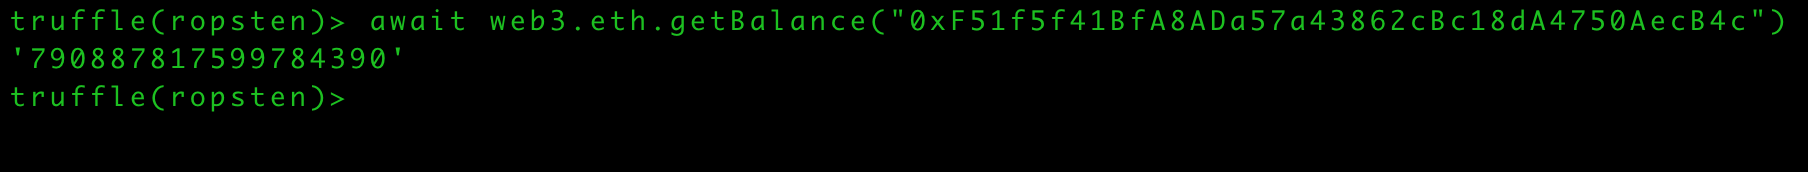
\includegraphics[width=12cm]{get-wallet-balance.png}}
\caption{دریافت موجودی کیف‌پول در خط فرمان ترافل}
\label{fig:get-wallet-balance}
\end{figure}


\subsection{دیپلوی قراردادهوشمند روی شبکه بلاکچین}
پس از اطمینان از توانایی پرداخت کارمزد تراکنش با استفاده از دستور migrate در خط فرمان ترافل قراردادهوشمند روی شبکه بلاکچین دیپلوی می‌شود.


\subsection{اطمینان از صحت دیپلوی قراردادهوشمند}
س از اتمام دیپلوی قرارداد هوشمند برای اطمینان از به درستی انجام شدن فرآیند دیپلوی قرارداد، می‌توان از
\glspl{Block Explorer}
بلاکچین استفاده کرد. برای مثال قرارداد هوشمند کاپو بر روی شبکه Ropsten دیپلوی شده است، که با رفتن به وبسایت اتراسکن
\LTRfootnote{
\url{https://etherscan.io}
}
و قراردادن آن روی شبکه Ropsten می‌توان قرارداد دیپلوی شده و تراکنش‌های آن را مشاهده کرد.


\begin{figure}[ht]
\centerline{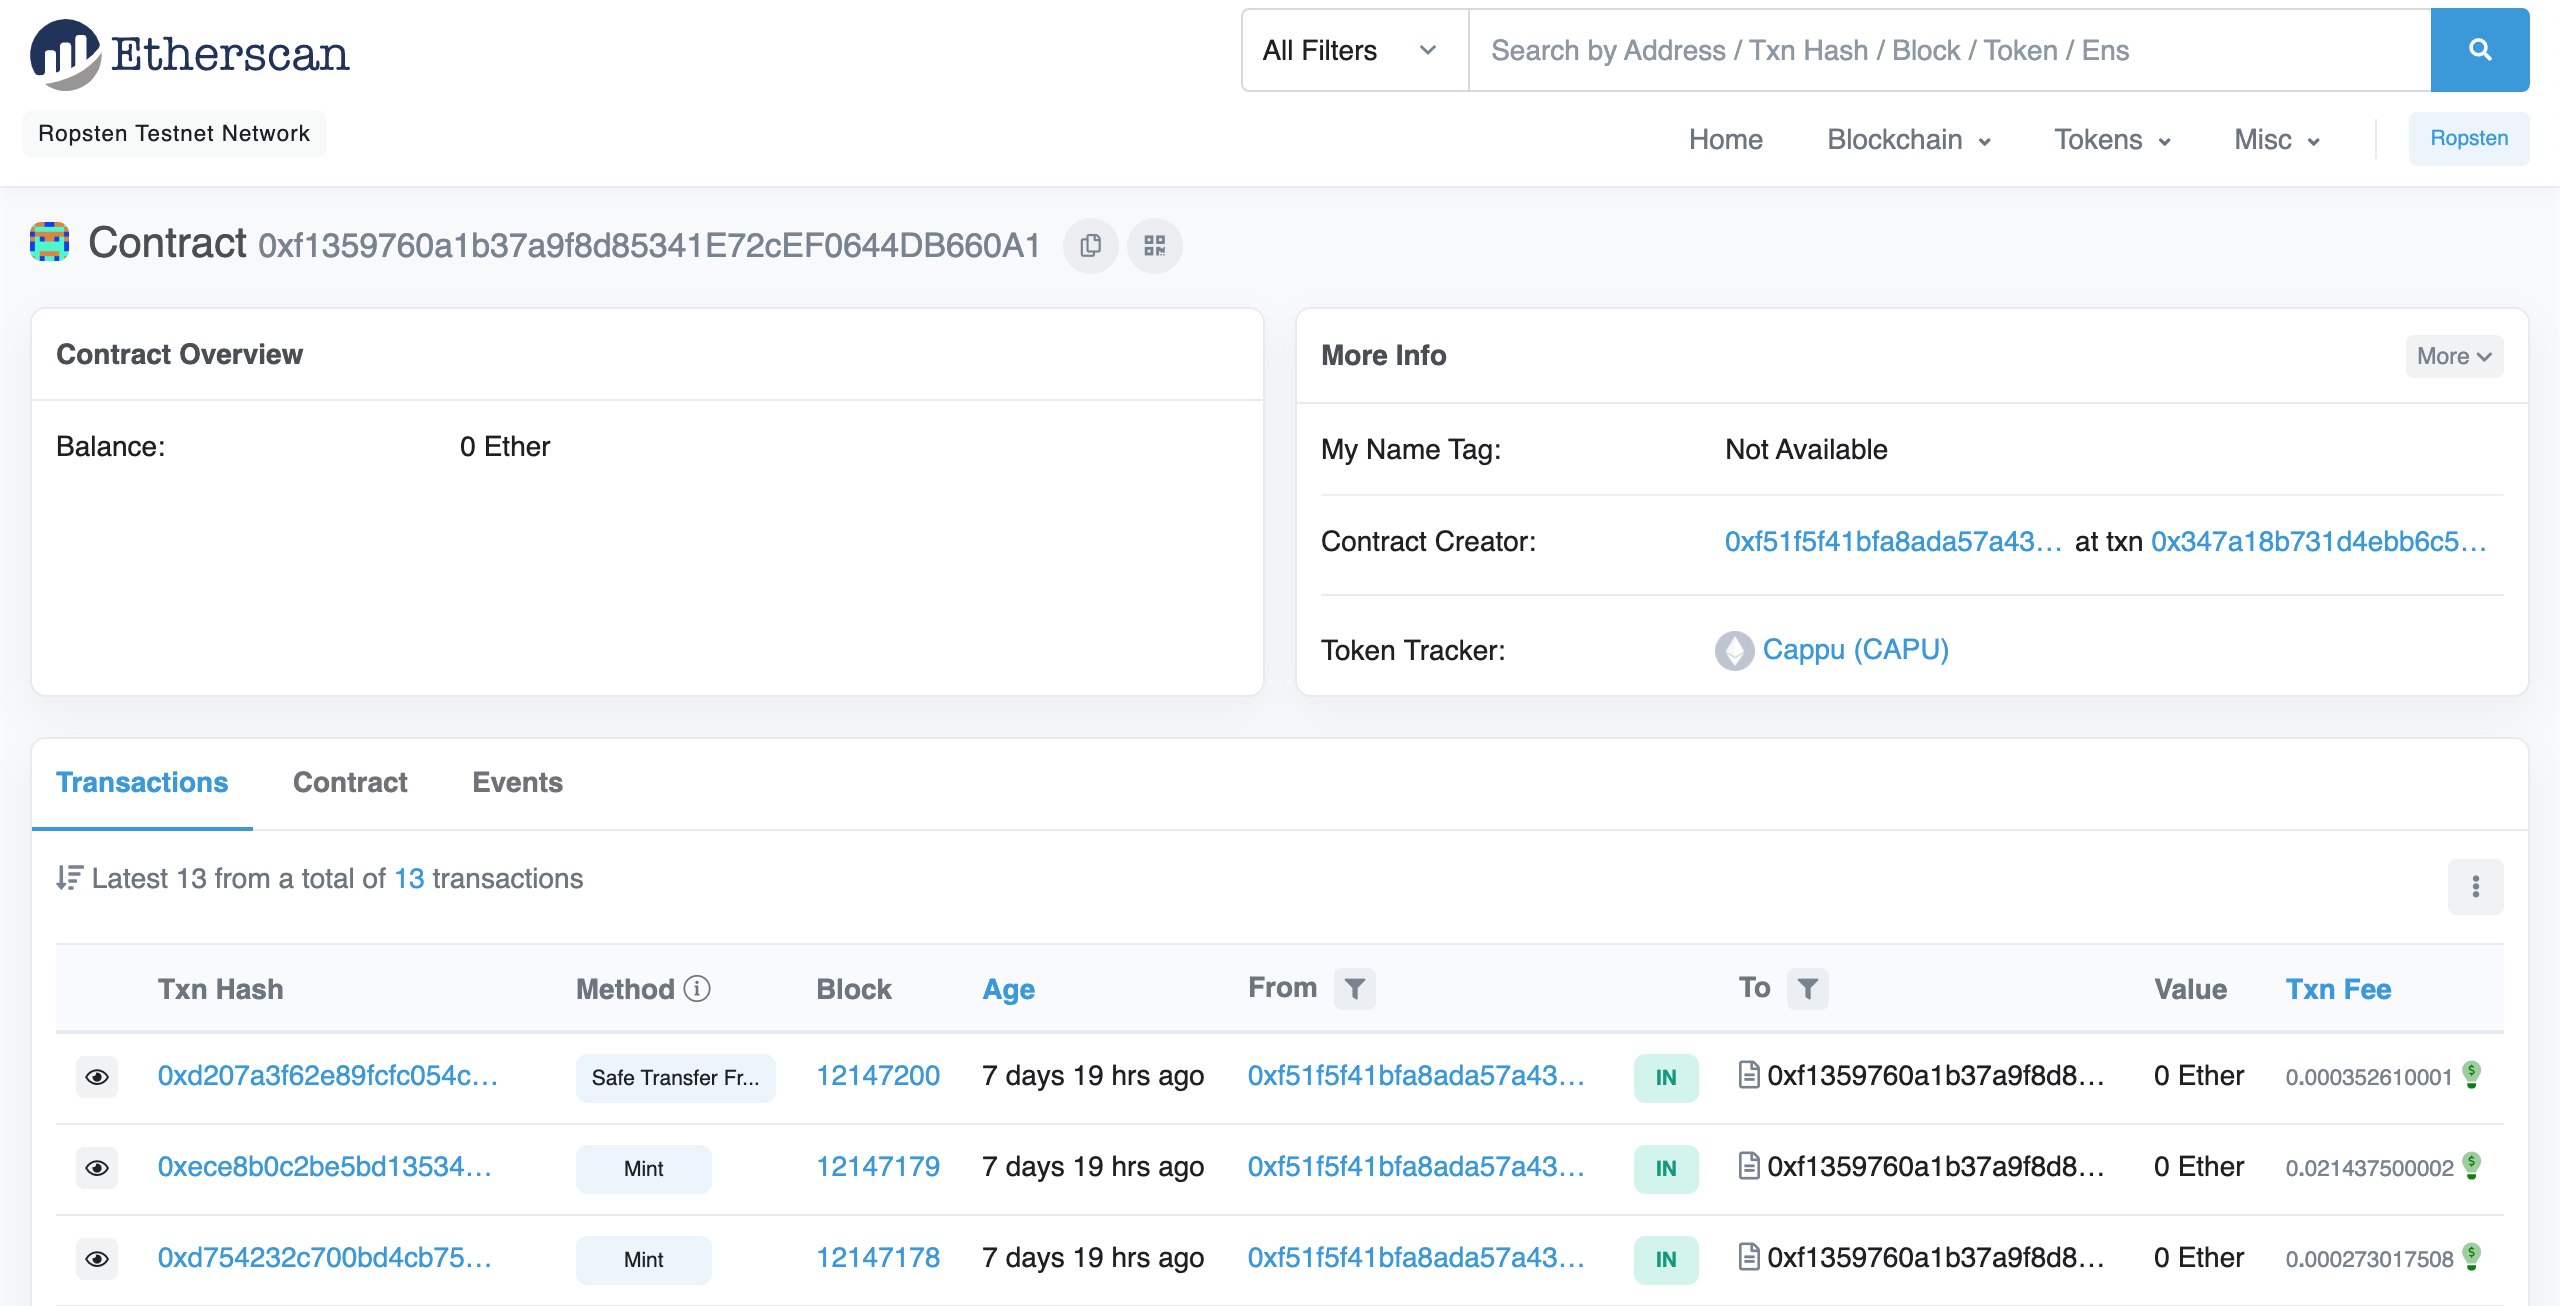
\includegraphics[width=12cm]{etherscan.png}}
\caption{مشاهده قراداد کاپو در Etherscan روی شبکه Ropsten}
\label{fig:etherscan}
\end{figure}


% ------------ Section 4.4
\section{توسعه فرانت، اتصال به قراردادهوشمند و فرآیند دیپلوی}
برای توسعه فرانت‌اند اپلیکیشن، React به عنوان چارچوب مورد استفاده انتخاب شد. ترکیب این چارچوب با استفاده از کتابخانه material-ui که کمک می‌کند در زمان کوتاه بتوان ظاهری زیبا و یکدست در اپلیکیشن ایجاد کرد و کتابخانه
\lr{Web3JS}
که فرانت‌اند را به کیف پول کاربر و شبکه بلاکچین متصل می‌کند، همه‌ی قابلیت‌های مورد نیاز برای توسعه یک فرانت‌اند زیبا و کارآمد را در اختیار توسعه دهنده قرار می‌دهد.

در پوشه اصلی فرانت‌اند فایلی با عنوان config.js وجود دارد. در این فایل علاوه بر ABI قراردادهوشمند سایر اطلاعات مورد نیاز مانند آدرس شبکه، آدرس قرارداد در شبکه و نام شبکه مورد نظر نیز ذخیره می‌شود. هنگام توسعه باید دقت شود که این فایل به قرارداد روی شبکه لوکال متصل شود.

برای استفاده از
\lr{Web3JS}
و اتصال به کیف‌پول کاربر یک فایل به نام connect.js ساخته شد، تمامی اعمال ارتباطی با کیف پول کاربر به عنوان چند تابع در این فایل جمع آوری شده‌اند، این فایل به صورت یک آداپتور میان
\lr{Web3JS}
و کد کاپو عمل می‌کند. تمامی قابلیت‌های مورد نیاز مانند اتصال به کیف‌پول و
\gls{Login}
کاربر،
\gls{Logout}
کاربر، گرفتن آدرس و شبکه‌ی کیف پول و ... در این فایل انجام می‌شود.

فرانت‌اند کاپو پس از تایید کاربر و دریافت آدرس کیف‌پول او، آن را در sessionStorage ذخیره می‌کند، از این طریق متوجه می شود که آیا کاربر وارد شده است یا خیر و با چه آدرسی. کاپو پیش از اتصال به کیف پول کاربر چک می‌کند که کیف پول روی شبکه یکسانی با شبکه فعلی کاپو باشد و در غیر این صورت به کاربر هشدار می‌دهد. همچنین در فرانت‌اند کاپو برای داشتن تجربه کاربری بهتر تلاش شده است. نکاتی مانند عدم نمایش قابلیت‌هایی مانند ساخت و ارسال توکن هنگامی که کیف پول کاربر به اپلیکیشن متصل نیست، جابه‌جایی آسان میان صفحات به کمک react-router، طراحی responsive برای رایانه و گوشی موبایل، نمایش alert ها و error های مناسب به کاربر، نمایش loading هنگامی که تراکنش‌ها در حالت pending هستند و نمایش پیام‌های مناسب با توجه به نتیجه تراکنش‌های کاربر.

برای این که کاربرها بتوانند با قراردادهوشمند ارتباط برقرار کنند نیاز است که فرانت‌اند اپلیکیشن در سروری بارگذاری شود. خوشبختانه گیت‌هاب قابلیت به نام
\lr{Github Pages}
در اختیار کاربرانش قرار می‌دهد که به کمک آن می‌توان فرانت‌اند اپلیکیشن را در آدرسی متناسب با آدرس مخزن کد در گیت‌هاب بارگذاری کرد و کاربران با رجوع به آن آدرس می‌توانند فرانت‌اند اپلیکیشن را ببینند و از آن استفاده کنند.

این قابلیت گیت‌هاب در واقع به این صورت عمل می‌کند که یک برنچ به نام gh-pages در repository پروژه می‌سازد و هربار که دستور دیپلوی پروژه توسط گیت‌هاب اجرا می‌شود، یک بیلد از پروژه می‌گیرد و فایل‌های خروجی بیلد روی این برنچ پوش می‌شوند. سپس این فایل‌ها روی آدرسی متناسب با آدرس repository دیپلوی می‌شوند. برای مثال آدرس ریپازیتوری و فرانت‌اند اپلیکیشن کاپو به صورت زیر است:
\begin{itemize}
  \item
  آدرس ریپازیتوری: \url{https://github.com/bshramin/cappu}
  \item
  آدرس فرانت‌اند: \url{https://bshramin.github.io/cappu}
\end{itemize}
البته دیپلوی شدن فرانت‌اند روی
\lr{Github Pages}
با ایجاد مشکلاتی در routing همراه بود که رفع شدند.


% ------------ Section 4.5
\section{داکرایز شدن، پایپلاین‌ها وگیت}
اقدامات زیر به منظور سرعت بخشیدن و تسهیل فرآیندهای توسعه و دیپلوی انجام شدند.

\subsection{داکرایز شدن تست‌های قراردادهوشمند}
برای سرعت بخشیدن به توسعه قراردادهوشمند، این نیازمندی به وجود آمد که بعد از پوش شدن هر تغییر روی گیت‌هاب تست‌های قرارداد به صورت خودکار اجرا شوند. به این منظور پیش از هر چیز تست‌های قراردادهوشمند باید بتوانند به صورت داکرایز اجرا شوند.

برای داکرایز کردن اجرای تست‌های قرارداد هوشمند، اول سعی در این بود که یک ایمیج داکر پایه که ترافل روی آن نصب شده باشد پیدا شود، اما نسخه ترافل نمونه‌هایی که یافت شد با نسخه مورد نظر همخوانی نداشت. در نتیجه یک ایمیج پایه داکر نوشته شد که داکرفایل آن را می‌توان در گیت‌هاب
\LTRfootnote{
  \url{https://github.com/bshramin/truffle-docker}
}
مشاهده کرد، همچنین این ایمیج داکر در داکرهاب
\LTRfootnote{
  \url{https://hub.docker.com/r/aminbshr/truffle}
}
نیز پوش شد.

سپس داکرفایل دیگری نوشته شد که با استفاده از این ایمیج پایه تست‌های قرارداد را اجرا کند. تست‌های قرارداد در این ایمیج که ترافل بر روی آن نصب شده است با اجرای دستور
\lr{truffle test}
اجرا می‌شود.


\subsection{اجرای خودکار تست‌های قرارداد}
با داشتن داکرفایلی که با بیلد و اجرای آن تست‌های قراردادهوشمند اجرا می‌شوند، تست‌های قراردادهوشمند می‌توانند به عنوان یکی از مراحل پایپلاین پروژه در گیت‌هاب نیز اجرا گردند. به این صورت در هر مرج ریکوئست به برنچ master و با پوش شدن یک کامیت در برنچ master تست‌ها به صورت خودکار در پایپلاین گیت‌هاب اجرا می‌شوند. به این ترتیب سرعت توسعه و اطمینان از کدهای قرارداد بیشتر می‌شود.


\subsection{دیپلوی خودکار فرانت‌اند}
برای ساده‌سازی بیشتر فرآیند دیپلوی فرانت‌اند و سرعت بخشیدن به توسعه آن، این قابلیت پیاده سازی می‌شود که پس از هربار ایجاد تغییر در فرانت‌اند، به جای این که توسعه‌دهنده با اجرای دستوراتی فرانت‌اند را به کمک
\gls{Github Pages}
دیپلوی کند، فرانت‌اند پس از پوش شدن تغییرات جدید روی برنچ اصلی ریپازیتوری دیپلوی می‌شود.

برای پیاده‌سازی این قابلیت از
\lr{Github Actions}
که در واقع پایپلاین‌های گیت‌هاب برای یک پروژه هستند استفاده می‌شود. تنها نکته‌ای که باید به آن توجه شود این است که این استیج از پایپلاین یک تفاوت اصلی با استیج‌های دیگر دارد. استیج‌های دیگر فقط می‌خواهند که کدهای ریپازیتوری را بخوانند و نمی‌خواهند چیزی را در ریپازیتوری تغییر دهند، اما این استیج می‌خواهد که کد‌های فرانت‌اند را بیلد کند و سپس فایل‌های بیلد شده را روی برنچ دیگری به نام gh-pages پوش کند. پس این استیج پایپلاین نیاز به دسترسی پوش کردن کد روی ریپازیتوری دارد.

برای پیاده‌سازی این قابلیت به این صورت عمل می‌شود که نخست یک داکرفایل نوشته می‌شود که در آن کدهای فرانت‌اند بیلد و سپس به کمک
\gls{Github Pages}
روی برنچ gh-pages پوش و دیپلوی می‌شوند. اما این کانتینر برای این که بتواند کدها را روی ریپازیتوری پوش کند نیاز به یک توکن از گیت‌هاب دارد، به همین دلیل برای این داکرفایل یک ENV تعریف می‌شود و هنگامی که در استیج دیپلوی فرانت‌اند این داکرفایل بیلد و اجرا می‌شود توکنی که از گیت‌هاب گرفته شده است به عنوان env به این کانتینر داده می‌شود. به این ترتیب این توکن درون کانتینر داکر وجود خواهد داشت و
\lr{Github Pages}
از آن استفاده خواهد کرد.

		% فصل چهارم: نتایج
% !TeX root=../main.tex
\chapter{دست‌آوردها، پیشنهاد‌ها، محدودیت‌ها}

\section{دست‌آوردها}

\subsection{یادگیری}
در طی انجام این پروژه با ابزارها، چارچوب‌ها، کتابخانه‌ها و استانداردهای توسعه قراردادهای هوشمند آشنا شدیم. آموختیم که چارچوب ترافل چه ابزارهایی را در اختیار توسعه دهنده قرار می‌دهد. چگونه می‌توان یک شبکه لوکال برای توسعه ایجاد کرد، قرارداد هوشمند را بر روی آن بارگذاری کرد و واسط کاربری و کیف پول را به آن متصل کرد.

آموختیم که چگونه می‌توانیم برای پیاده‌سازی قراردادهای هوشمند از استانداردهای موجود استفاده کنیم، برای آن‌ها تست بنویسیم و به کمک چارچوب ترافل این تست‌ها را اجرا کنیم. آموختیم که چگونه پس از اتمام فرآیند توسعه قراردادهوشمند را بر روی شبکه تستی بارگذاری کنیم. همچنین واسط کاربری اپلیکیشن به کمک صفحات گیت‌هاب بارگذاری و به قرارداد هوشمند روی شبکه تست متصل شد.

\subsection{پلتفرم ایجاد شده}
قرارداد هوشمند نوشته شده در این پروژه، کاپو، با عملکرد کامل بر بروی شبکه تستی Ropsten بارگذاری شد و امکانات لازم برای دسترسی عموم مردم به روشی آسان و ارزان به توکن‌های تعویض ناپذیر را فراهم می‌کند. کاربران می‌توانند در صفحه اصلی این اپلکیشن تعداد توکن‌های ساخته شده و تعداد آدرس‌های دارای توکن را مشاهده کنند. سپس با متصل کردن کیف‌پولشان به اپلیکیشن می‌توانند توکن بسازند، دارایی‌هایشان را مشاهده کنند و توکن‌هایشان رو به دیگران ارسال کنند.

\subsection{ساخت محیط توسعه سریع و خودکار}
سپس آموختیم که چگونه اجرای تست‌های قرارداد هوشمند را داکرایز و به صورت خودکار در پایپ‌لاین پروژه اجرا کنیم. برای انجام این کار یک داکر ایمیج ترافل نوشته شد، کد آن به صورت متن‌باز بر روی گیت‌هاب بارگزاری و ایمیج آن به داکرهاب اضافه شد. سپس واسط کاربری اپلیکیشن داکرایز شد و از env های داکر برای فرستادن توکن گیت‌هاب از پایپلاین به کانتینر استفاده شد و در نتیجه واسط کاربری اپلیکیشن به صورت خودکار در پایپلاین پروژه روی صفحات گیت‌هاب بارگزاری می شود.

در نتیجه انجام این کارها یک مسیر راحت و سریع برای توسعه یک قرارداد هوشمند به همراه واسط کاربری ایجاد شد که تست‌ها و فرایند بارگذاری همه به صورت خودکار در آن اجرا می‌شوند.



\section{پیشنهادها}
در این قسمت با توجه به آموخته‌هایی که در طی انجام این پروژه به دست آمد،
پیشنهادهایی برای توسعه پروژه‌های مشابه ذکر می شود.
امید است که استفاده از این پیشنهادها مسیر توسعه را هموارتر کرده و سرعت ببخشد.

\subsection{استفاده از استانداردها}
خوشبختانه در این پروژه از ابتدا به استفاده از استانداردهای موجود اهمیت داده شد.
در صورتی که توسعه دهنده بخواهد از استانداردهای موجود استفاده نکند مزیت سازگاری
قرارداد هوشمند نوشته شده با پلتفرم‌هایی که از پیش وجود دارند را از دست می‌دهد.

همچنین در صورتی که توسعه دهنده تصمیم بگیرد که از یکی از استانداردها پیروی کند
بهتر است که از پیاده‌سازی‌های موجود به صورت متن‌باز استفاده کند، این تصمیم باعث
رشد چشمگیر سرعت توسعه قرارداد هوشمند می‌شود، امکان وجود خطا و مشکل امنیتی در قرارداد را کم
و امکان دریافت آپدیت‌های جدید را تسهیل می‌کند.


\subsection{استفاده از \lr{ERC1155} به جای \lr{ERC721}}
استاندارد
\lr{ERC1155}
برتری‌های فراوانی نسبت به استاندارد
\lr{ERC721}
دارد.
از جمله این برتری‌ها می‌توان به قابلیت ارسال چند توکن در یک تراکنش،
توانایی ساخت انواع مختلف توکن با تعداد متفاوت و
پشتیبانی از توکن‌های تعویض‌پذیر و تعویض‌ناپذیر به صورت همزمان اشاره کرد.
با توجه به قابلیت ارسال هم‌زمان چند توکن و یا ساخت هم‌زمان چندین توکن در یک تراکنش، هزینه‌ی پرداختی کاربرها نیز
برای استفاده از قرارداد هوشمند به نحو شایانی کاهش می‌یابد و به این نحو قرارداد در دسترس
جامعه بزرگتری قرار می‌گیرد.

\subsection{ساخت محیط توسعه از شروع کار}
انجام مواردی مانند خودکار سازی اجرا شدن تست‌ها، بارگذاری رابط کاربری و استفاده از ابزارهای کنترل ورژن مانند گیت‌هاب
گرچه در شروع کار ممکن است خسته‌کننده باشند و به توسعه‌دهنده حس پیشرفت در انجام پروژه را ندهند، اما
این کارها هرچه زودتر و در شروع پروژه انجام شوند سرعت پیشرفت پروژه را دو چندان می‌کنند.
در نتیجه پیشنهاد می‌شود که در نقطه شروع پروژه به روند توسعه توجه شود و زمانی به
بهینه‌سازی این روند اختصاص داده شود.


\section{محدودیت‌ها}

\subsection{استفاده از \lr{Drizzle}}
در ابتدای انجام پروژه سعی شد که برای برقراری ارتباط رابط کاربری با قرارداد هوشمند از
\gls{Drizzle}
استفاده شود.
اما استفاده از این ابزار مشکلات فراوانی را به همراه داشت.
با توجه به تازگی و بالغ نبودن ابزارهای موجود برای توسعه قراردادهای هوشمند،
باید سعی شود که تا جای ممکن از ابزارهای پراستفاده و با
\gls{Community}
بزرگ استفاده شود. در این پروژه پس از مواجهه با محدودیت‌های فراوان دریزل،
از کتابخانه‌ \lr{Web3JS} استفاده شد که دست توسعه دهنده را به میزان خوبی باز می‌گذارد.

\subsection{ورژن‌های مختلف ابزارها}
عدم همخوانی نسخه‌های مختلف ابزارهای مورد استفاده با یکدیگر مشکلات زیادی در توسعه پروژه ایجاد کرد.
در هنگام توسعه پروژه باید حتما دقت شود که برای هر ابزار در حال استفاده از چه نسخه‌ای هستیم.
همچنین برای محدود کردن این مشکل پیشنهاد می‌شود از ابزارهای کانتینر کننده مانند داکر استفاده شود.

\subsection{هزینه تراکنش‌های شبکه اصلی اتریوم}
در زمان نوشته شدن این متن، هزینه انجام تراکنش روی شبکه اصلی اتریوم به شدت بالاست.
این هزینه‌ی بالا باعث می‌شود که بارگذاری کردن روی شبکه اصلی برای یک پروژه آزمایش از دسترس دور باشد.
اگرچه ممکن است در آینده با بروزرسانی اتریوم ۲ این هزینه به شدت کاهش یابد.

\subsection{عدم وجود راهنما و مستندات کافی}
تازگی این زمینه باعث عدم وجود راهنما و مستندات کافی شده است.
این موضوع از دیگر دلایل پیشنهاد به استفاده از ابزارهای با جامعه توسعه‌دهندگان بزرگ است.
		% فصل پنجم: بحث و نتیجه‌گیری

% مراجع
% اگر از استیل‌های natbib استفاده می‌کنید باید دو خط را در فایل commands.tex تغییر دهید.
\pagestyle{empty}
{
\small
\onehalfspacing
\bibliographystyle{plain-fa} % or plainnat-fa for author-date
\bibliography{./tex/MyReferences}
}

\pagestyle{fancy}

% \appendix
% فصلهای پس از این قسمت به عنوان ضمیمه خواهند آمد.

% دستورات لازم برای تبدیل «فصل آ» به «پیوست آ» در فهرست مطالب
\addtocontents{toc}{
    \protect\renewcommand\protect\cftchappresnum{\appendixname~}%
    \protect\setlength{\cftchapnumwidth}{\mylenapp}}
    
% دستورات لازم برای شماره‌گذاری صفحات پیوست‌ها بشکل آ-۱ (فعلا با glossaries سازگار نیست)
% \let\Chapter\chapter
%\pretocmd{\chapter}{
%  \clearpage
%  \pagenumbering{arabic}
%  \renewcommand*{\thepage}{\rl{\thechapter-\arabic{page}}}}{}{}
%%%%%%%%%%%%%%%%%%%%%%%%%%%%%%%%%%%%%
        

% \include{./tex/appendix1}		% پیوست اول: آشنایی مقدماتی با لاتک
% \include{./tex/appendix2}		% پیوست دوم: جدول، نمودار و الگوریتم در لاتک
% \include{./tex/appendix3}   	% پیوست سوم: مراجع، واژه‌نامه و حاشیه‌نویسی

% برگرداندن شماره‌بندی صفحات فصول
% \let\chapter\Chapter
\pagenumbering{tartibi} % اول، دوم، ...
%\baselineskip=.75cm

% چاپ واژه‌نامه‌ها و نمایه 
% \onehalfspacing
% \cleardoublepage
% \printglossary
% \cleardoublepage
% \printindex

\begin{latin}
\baselineskip=.6cm
\latinabstract
\latinTitlePage
\end{latin}
\label{LastPage}

\end{document}
